\documentclass[fleqn,10pt]{wlpeerj}
\title{Simulation of Brain Functional Connectivity on Empirical and Randomized Brain Structural Networks}

\usepackage{color} 
\newcommand{\red}[1]{\textcolor{red}{(#1)}}
\newcommand{\reg}[1]{~ \\ \textcolor{red}{\framebox{\begin{minipage}{0.9\linewidth}\footnotesize\em
#1  \end{minipage}}}\\}

\author[1]{\c{S}eyma \textsc{Bayrak}}
\author[2,3]{Vesna \textsc{Vuksanovi\'c}}
\author[2,3]{Philipp \textsc{H\"{o}vel}}

\affil[1]{Institute of Biology, Otto-von-Guericke-Universit{\"a}t Magdeburg, Leipziger Stra{\ss}e 44, 39120 Magdeburg,
Germany}
\affil[2]{Institut f{\"u}r Theoretische Physik, Technische Universit\"at
Berlin, Hardenbergstra\ss{}e 36, 10623 Berlin, Germany }
\affil[3]{Bernstein Center for Computational Neuroscience Berlin, Humboldt-Universit{\"a}t zu Berlin, Philippstra{\ss}e 13, 10115 Berlin, Germany }


\keywords{resting state, functional and anatomical connectivity, time-delayed oscillations, hemodynamic model, brain networks}

\begin{abstract}
% Blood oxygen level dependent (BOLD) contrast imaging is one of the widely used fMRI techniques to map the brain activity at resting-state, i.e. in the absence of any stimulus-driven task.  The BOLD fluctuations arising from changing neuronal activity at resting-state have been observed to be complex but highly structured and robust. A well-explored BOLD response in the brain would potentially lead to easier diagnosis of neurodegenerative disorders such as Alzheimer's disease and Parkinson's disease. However, the underlying biophysical mechanism of the resting-state activity of the brain has not yet been completely uncovered.
This study combines experimental and modeling approaches in order to investigate the temporal dynamics of the human
brain at rest. The dynamics of the neuronal activity is modeled with FitzHugh-Nagumo oscillators and the blood-oxygen-level-dependent (BOLD)
time-series is inferred via the Balloon-Windkessel hemodynamic model. The simulations are based on structural connections
that are derived from diffusion-weighted magnetic resonance imaging measurements yielding anatomical probabilities
between the considered brain regions of interest. In addition, the length of the fiber tracks allows for inference of
the coupling delays due to finite signal propagation velocities. We aim to (i) investigate the network topology of
structural connectivity by comparing it to random graphs, (ii) demonstrate  how functionally correlated BOLD signals
emerge from the anatomical connections, and (iii) explore how the dynamics simulated on empirical brain networks differs
from the dynamics on randomized networks.
\end{abstract}

\begin{document}
% \flushbottom
\maketitle
% \thispagestyle{empty}

\section*{Introduction}
Large-scale functional brain connectivity maps are networks of brain regions based on functional interactions, i.e.
co-activation between these regions \citep{BIS95, BRE10b, DAM06}. In a typical functional magnetic resonance imaging
(fMRI) experiment, functional connections are obtained from brain regions, whose corresponding time series of
blood-oxygen-level-dependent (BOLD) activity display significant correlations at low-frequencies ($< 0.1$ Hz). Well
organized spatio-temporal low-frequency fluctuations have been reported in BOLD-fMRI signals of a mammalian brain at
rest, i.e. in the absence of any stimulation-driven task \citep{BIS95, DAM06, VIN07a}. Despite important progress over
the past few years, the way how functional connectivity arises from complex anatomical connectivity still remains
poorly understood \citep{GHO08, DEC09, CAB12, CAB14, VUK14}.

Existing models of resting-brain dynamics hypothesize that functional interactions result from a complex interplay
between intrinsic brain dynamics and underlying structural connections \citep{HAG08, GHO08, RUB09, DEC12, VUK13}.
Previously, the neuronal dynamics have been modeled as coupled nonlinear oscillators \citep{WIE61, LOP97, NUN98, NUN00,
PO08}, Hopf oscillators \citep{JIR07}, Wilson-Cowan systems \citep{DEC09}, FitzHugh-Nagumo systems \citep{GHO08, VUK13},
and Kuramoto oscillators \citep{BRE10i, VUK14}. In particular, these models explore the range of conditions at which
functional networks emerge from anatomical connections: the role of multiple time-scales in the formation of functional
connectivity networks \citep{HON07}, time delays in the signal propagation between the network nodes as well as the
system noise \citep{GHO08, GHO08a}, local network oscillations \citep{DEC09, CAB11}, and structural disconnection
\citep{CAB12}.

Our investigation provides a deeper insight to the relation between functional and anatomical brain connectivity: how
is the dynamical process of brain's functional connectivity shaped by its structural topology? The considered networks
are constructed from an anatomical connectivity (AC) map via binarization. For comparison, we also construct random
networks by manipulating the AC map to obtain random networks of Erd\H{o}s-R\'{e}nyi type \citep{XYZERD}. The neuronal
activity and the BOLD fluctuations are simulated on both network types by the FitzHugh-Nagumo (FHN) model as proposed in
\citep{GHO08, GHO08a, VUKnew} and the Balloon-Windkessel hemodynamic model \citep{FRI00}, respectively. As system parameters, we
vary the network density and the strengths of the delayed coupling. Purpose of the study is: (i) to analyze the similarities and differences in the network topologies
of structural brain networks and corresponding random graphs, (ii) to compare the simulated functional BOLD fluctuations
based on AC maps with empirical functional connectivity (FC), and (iii) to explore 
how the simulated temporal dynamics of brain networks differ from the dynamics based on random networks.
% the parameter space of $(p,c)$, where  $c$ denotes the coupling strength of the FHN network model. 

The rest of this paper is organized as follows: In Sec. Materials \& Methods, we introduce the empirical data sets of FC
and AC maps and describe the construction scheme of brain graphs based on AC maps and corresponding random graphs. The
temporal dynamics of the network nodes emerge from the FHN model and the Balloon-Windkessel hemodynamic model for the
neuronal dynamics and BOLD time series, respectively \citep{FIT61, FRI00}. The section  closes
with a summary of the statistical approaches used to compare the empirical and simulated data sets. In Sec. Results \&
Discussion, we compare network characteristics of brain and random graphs. Then, we discuss the simulated BOLD
fluctuations modeled on the structural brain network and compare them to the empirical FC map. Finally, we analyze the
similarity between the modeled temporal dynamics on brain graphs and that on random networks. Finally, Sec. Conclusion
summarizes the key findings.
% : it is possible to explore such regions on parameter space $(p,c)$, where \textit{i)} 
% BOLD fluctuations are captured through structural brain connections, and \textit{ii)} temporal dynamics of brain graphs are different from that of random graphs. 
 
\section*{Materials \& Methods}
\subsection*{Empirical Brain Connectivity Maps}
The resting-state FC and AC maps in the present study are taken from \cite{VUK14}. The AC map is obtained
from diffusion-weighted magnetic resonance imaging (DW-MRI) measurements of \cite{ITU08}. The obtained network is based
on $N=90$ cortical and sub-cortical regions (\textit{nodes}) defined by automated anatomic labeling (AAL) method
\citep{TZO02}. Within the AAL template, the indexes $1, 2, \dots ,45$ refer to the right hemisphere  and regions labeled
$46,47, \dots ,90$ correspond to the left hemisphere (Table \ref{tab:AAL}). The values in the AC matrix refer to the
probability of two AAL regions being connected at least by a single nervous fiber. 

The FC map is derived from the \textit{1000 Functional Connectome Project} website \textit{http://www.nitric.org/} according to the procedure described in \cite{VUK14}. It is based on the same AAL template as the AC map. The FC matrix represents the Pearson correlations between BOLD signals of any two AAL regions \citep{MARG07, VUK14}.

\begin{figure}[ht]\centering
 \includegraphics[width=0.49\textwidth]{Figures/cor_FCM_exp} 
 \includegraphics[width=0.49\textwidth]{Figures/cor_ACM_exp} 
 \caption{Empirical functional and anatomical connectivity maps of human cortex: FC map obtained from fMRI-BOLD
technique (left) and AC map obtained from DW-MRI measurements (right). The color bars show correlation coefficients and
probability values in the FC and AC map, respectively.}
\label{fig:Empirical FCM and ACM}
\end{figure}

Figure~\ref{fig:Empirical FCM and ACM} depicts the empirical FC and AC matrices.
% All correlation coefficients
% in FC map are in the range [0,1] as well as all probability values in AC map. 
Both matrices are symmetric. A
correlation value close to 1 in the FC matrix indicates that the functional activities of the respective nodes
highly resemble each other. See, for instance, the sub-diagonals in Figure~\ref{fig:Empirical FCM and ACM} (left) with
strong correlation between corresponding brain regions in both hemispheres. A probability value
close to 1 in AC matrix demonstrates that involved nodes are most likely connected by fiber tracks in the white
matter. Although some node pairs are not anatomically coupled at all in AC map (cold colors), they could be functionally
coupled in FC map (hot colors).
% This is especially true for the corresponding regions in the different hemispheres.    

% \begin{figure}[ht]\centering
% 	 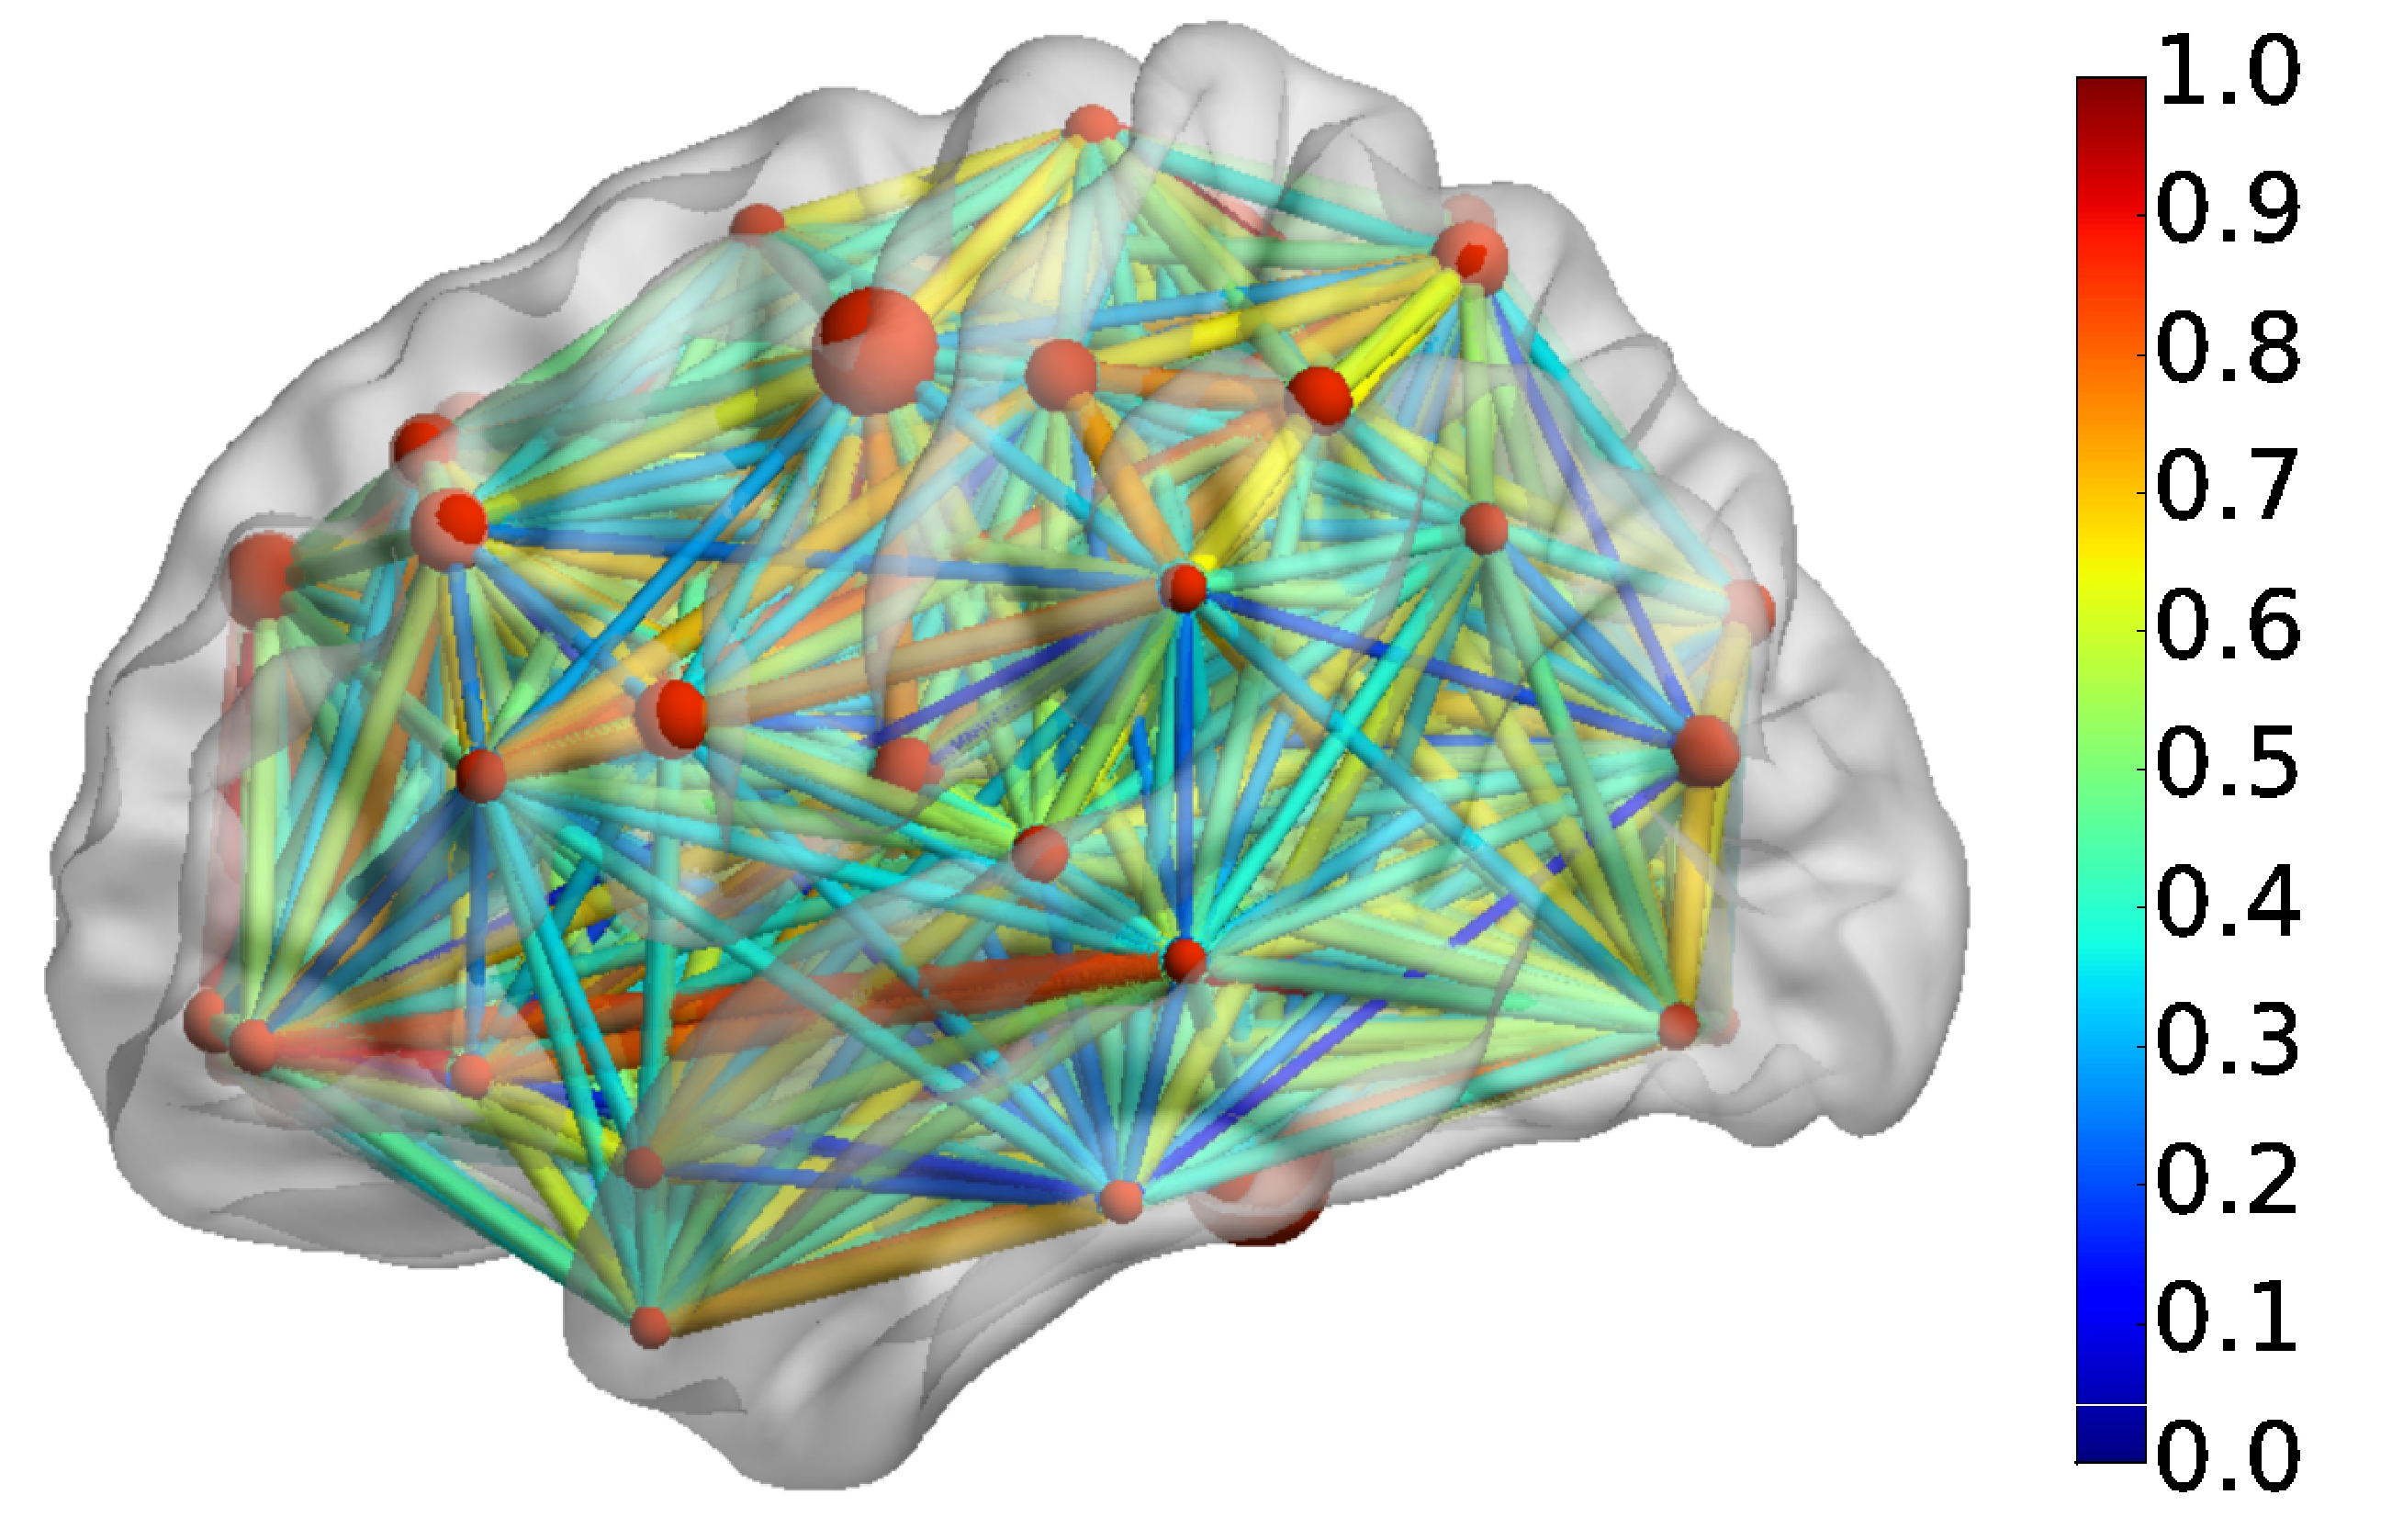
\includegraphics[width=0.49\textwidth]{Figures/FCM_brain} 
% 	 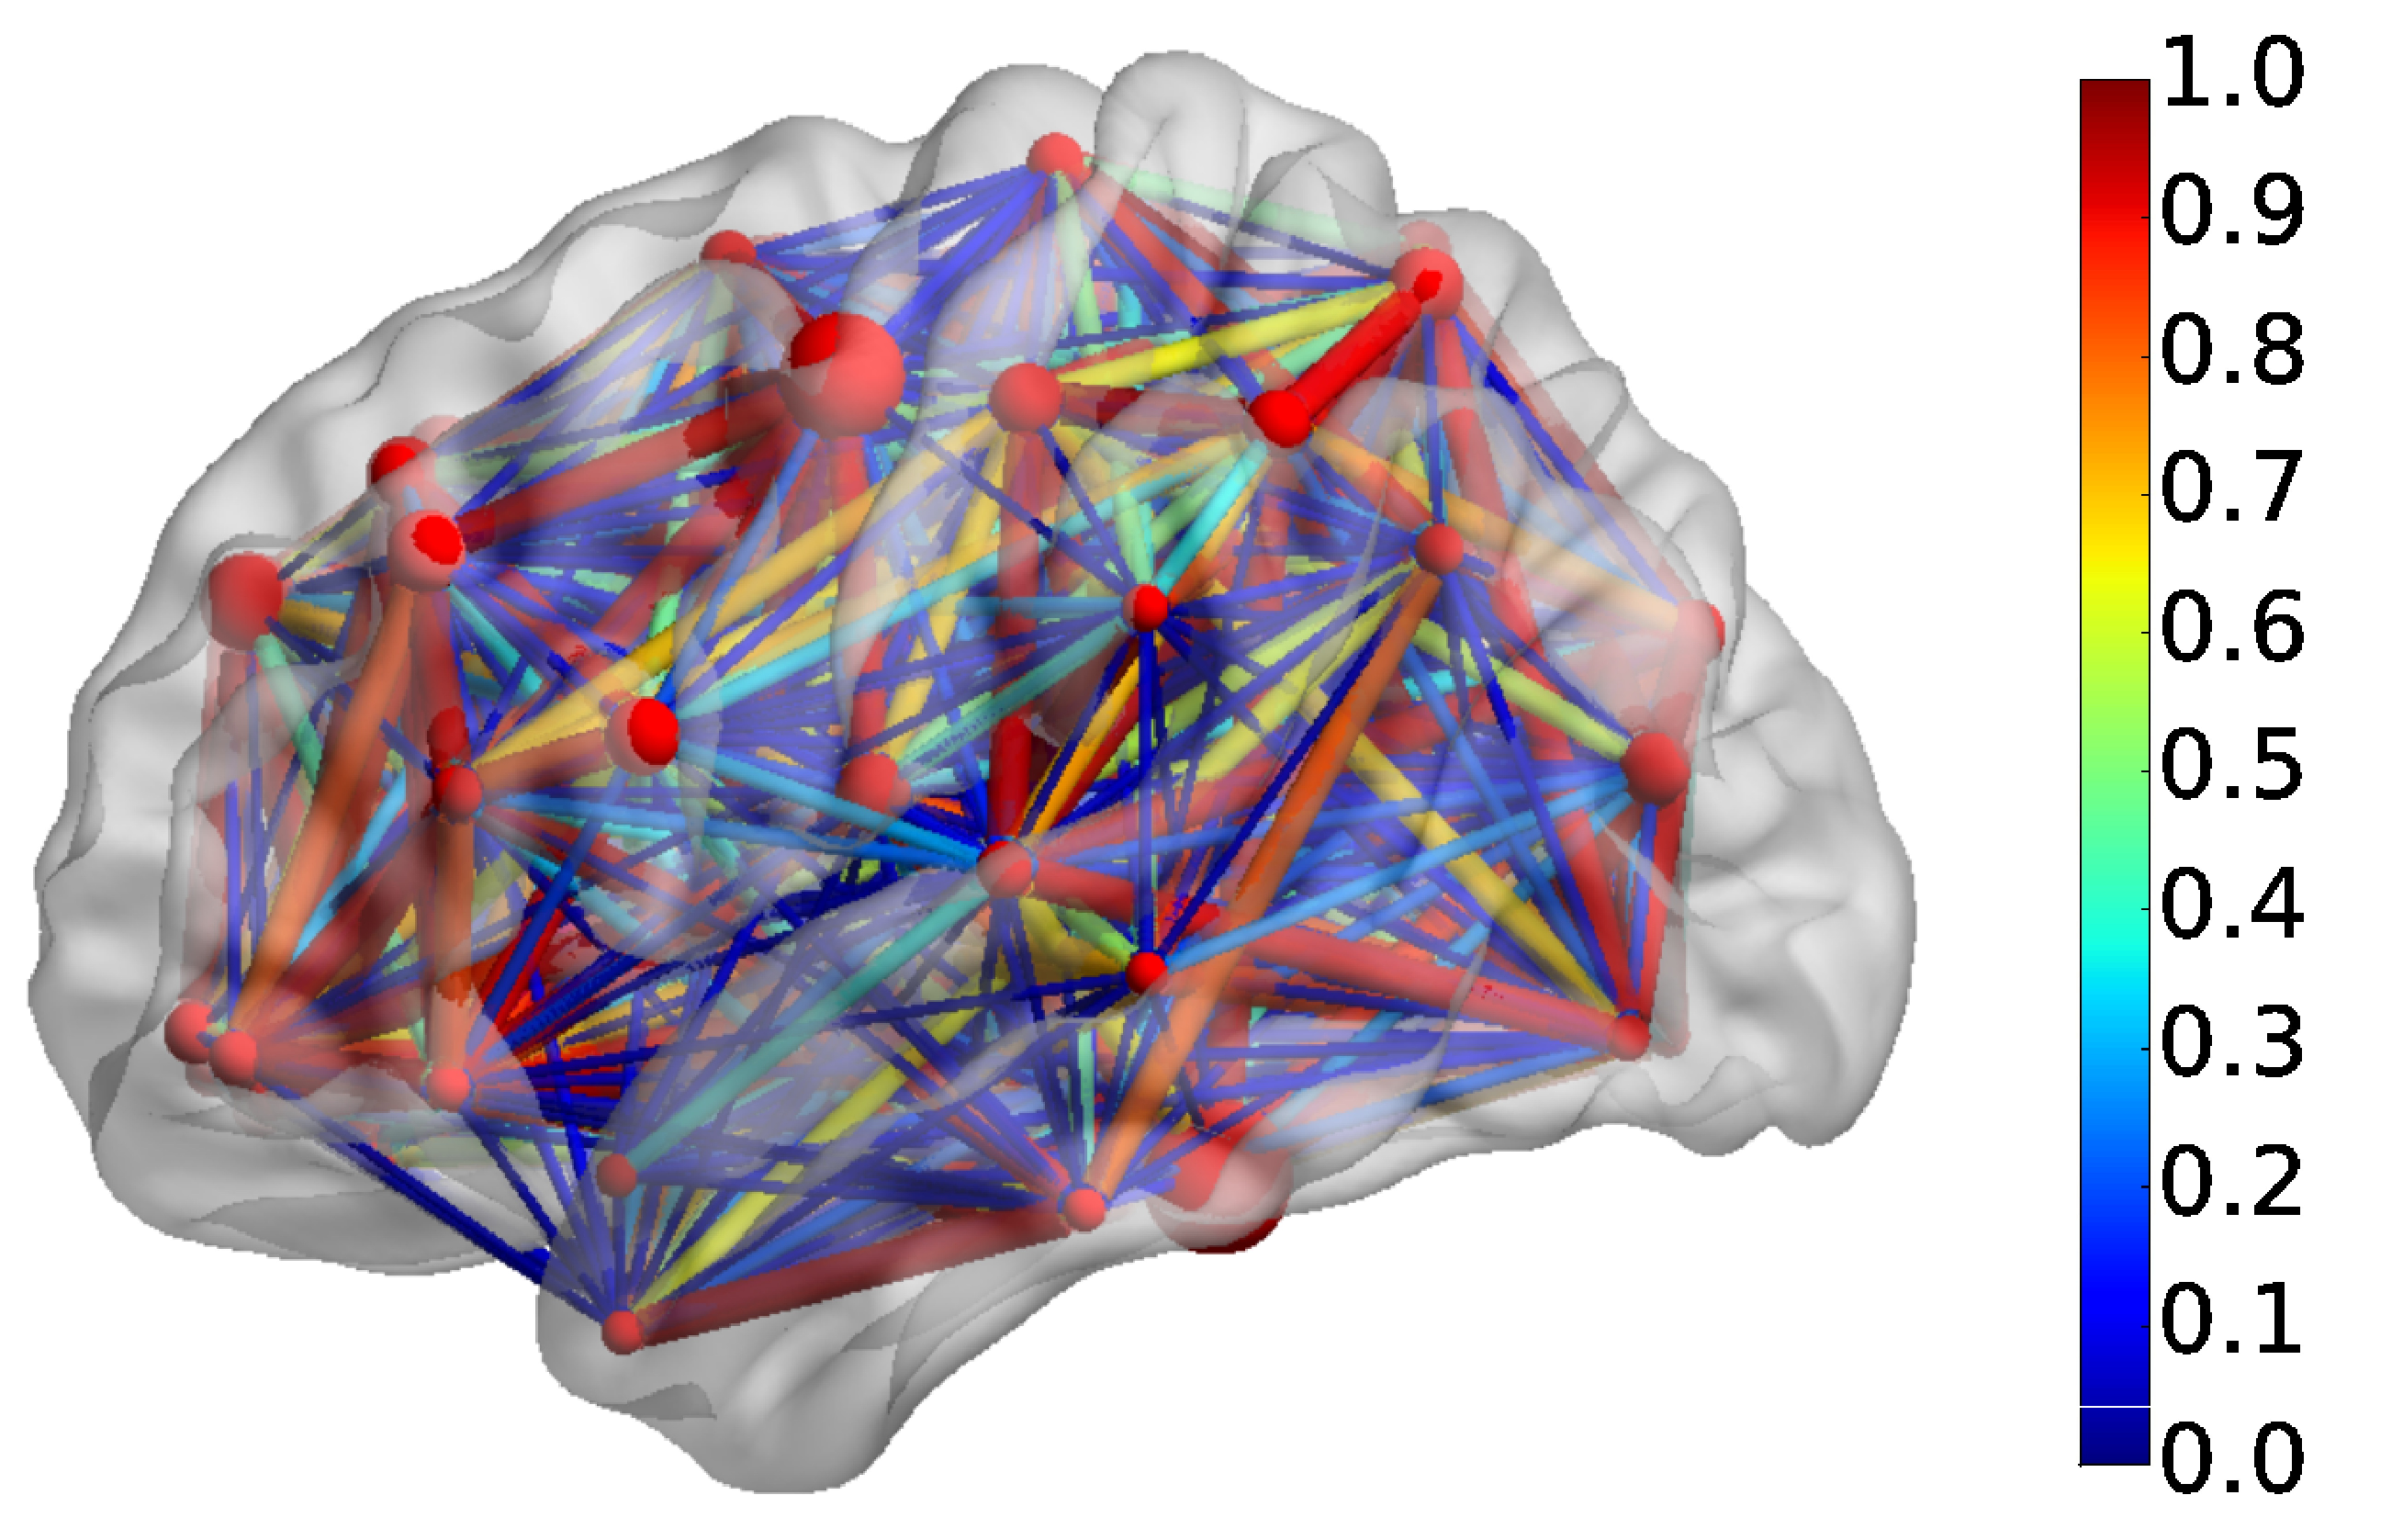
\includegraphics[width=0.49\textwidth]{Figures/ACM_brain} 
% \caption{3D sagittal visualization of empirical FC (left) and AC  maps (right) on the human cortex with the
% \textsc{BrainNet Viewer} \citep{XYZ13}. The color bars are the same as explained in Figure~\ref{fig:Empirical FCM and
% ACM}.  }
% \label{fig:Empirical FCM and ACM in Cortex}
% \end{figure}
% 
% FC and AC matrices presented in Figure~\ref{fig:Empirical FCM and ACM} are embedded in human cortex in Figure
% \ref{fig:Empirical FCM and ACM in Cortex} \citep{XYZ13}. The AAL regions are presented by red colored nodes with varying
% size dependent of \textit{nodal degree}. The \textit{edges} have different thickness and color distribution according to
% correlation coefficients and probability values with respect to FC and AC maps. The nerve fibers between nodes exist
% either with high (hot colors) or low (cold colors) probability (Figure~\ref{fig:Empirical FCM and ACM in Cortex},
% right). However, the functional correlations (Figure~\ref{fig:Empirical FCM and ACM in Cortex}, left) tend to have an
% intermediate value (green colors). The distribution of anatomical and functional connections are clearly distinguishable
% in human brain.   

\subsection*{The Brain Graph and Erd\H{o}s-R\'{e}nyi-Type Random Graph}

% \paragraph{The Brain Graph}
The brain graphs considered in the present study are generated by binarizing the empirical AC map via thresholding, that
is, we define a threshold value for
the connection probability $p$ of node pairs. Then, the values greater and equal to $p$ are set to 1 in the
connectivity matrix and to 0 otherwise. This way, the resulting binary \textit{adjacency matrix} reflects the coupling
topology of the brain graphs, which are treated as \textit{undirected} and \textit{unweighted} networks. In other words,
all existing edges are thought to be of uniform weight and nodes interact both ways along an edge connecting them. 
% Neither the direction of anatomical connectivity between nodes
% nor any other values apart from 0 and 1  are encoded in the adjacency matrices so that 

% \reg{PH: CONTINUE FROM HERE}
% \paragraph{Erd\H{o}s-R\'{e}nyi-Type Random Graph}
In order to compare the effects of network structure of the brain graph with a generic network, we construct reference
networks with the same \textit{network density} $\kappa$ in the form of random graphs. This follows a construction
first discussed by Paul Erd\H{o}s and Alfr\'{e}d R\'{e}nyi in their seminal paper  \citep{XYZERD}. Given a total number
of nodes $N$ and total number of edges $L$, so-called Erd\H{o}s-R\'{e}nyi networks are undirected graphs $G(N,P)$, in
which the presence of any edge between two nodes is realized with a fixed probability $P$. This results in a
binomial distribution for the number of edges per node, known as the \textit{degree}.  A particular graph $G(N,P)$ is
chosen uniformly random out of the set of all potential graphs having $N$ nodes and $L$ edges, which means the same
\textit{network density} $\kappa$. The probability for a graph to be picked among all the others is $L/\binom
{N}{2}$ \citep{NEW10}. 

In this study, we denote brain graphs as $R_{BG}$ and Erd\H{o}s-R\'{e}nyi-type random graphs as $R_{ER}$ for
notational convenience. For an analysis of these graphs, we use the \textsc{NetworkX} software package implemented in
\textsc{PYTHON} \citep{XYZNETW}.

\begin{figure}[htpb]\centering
	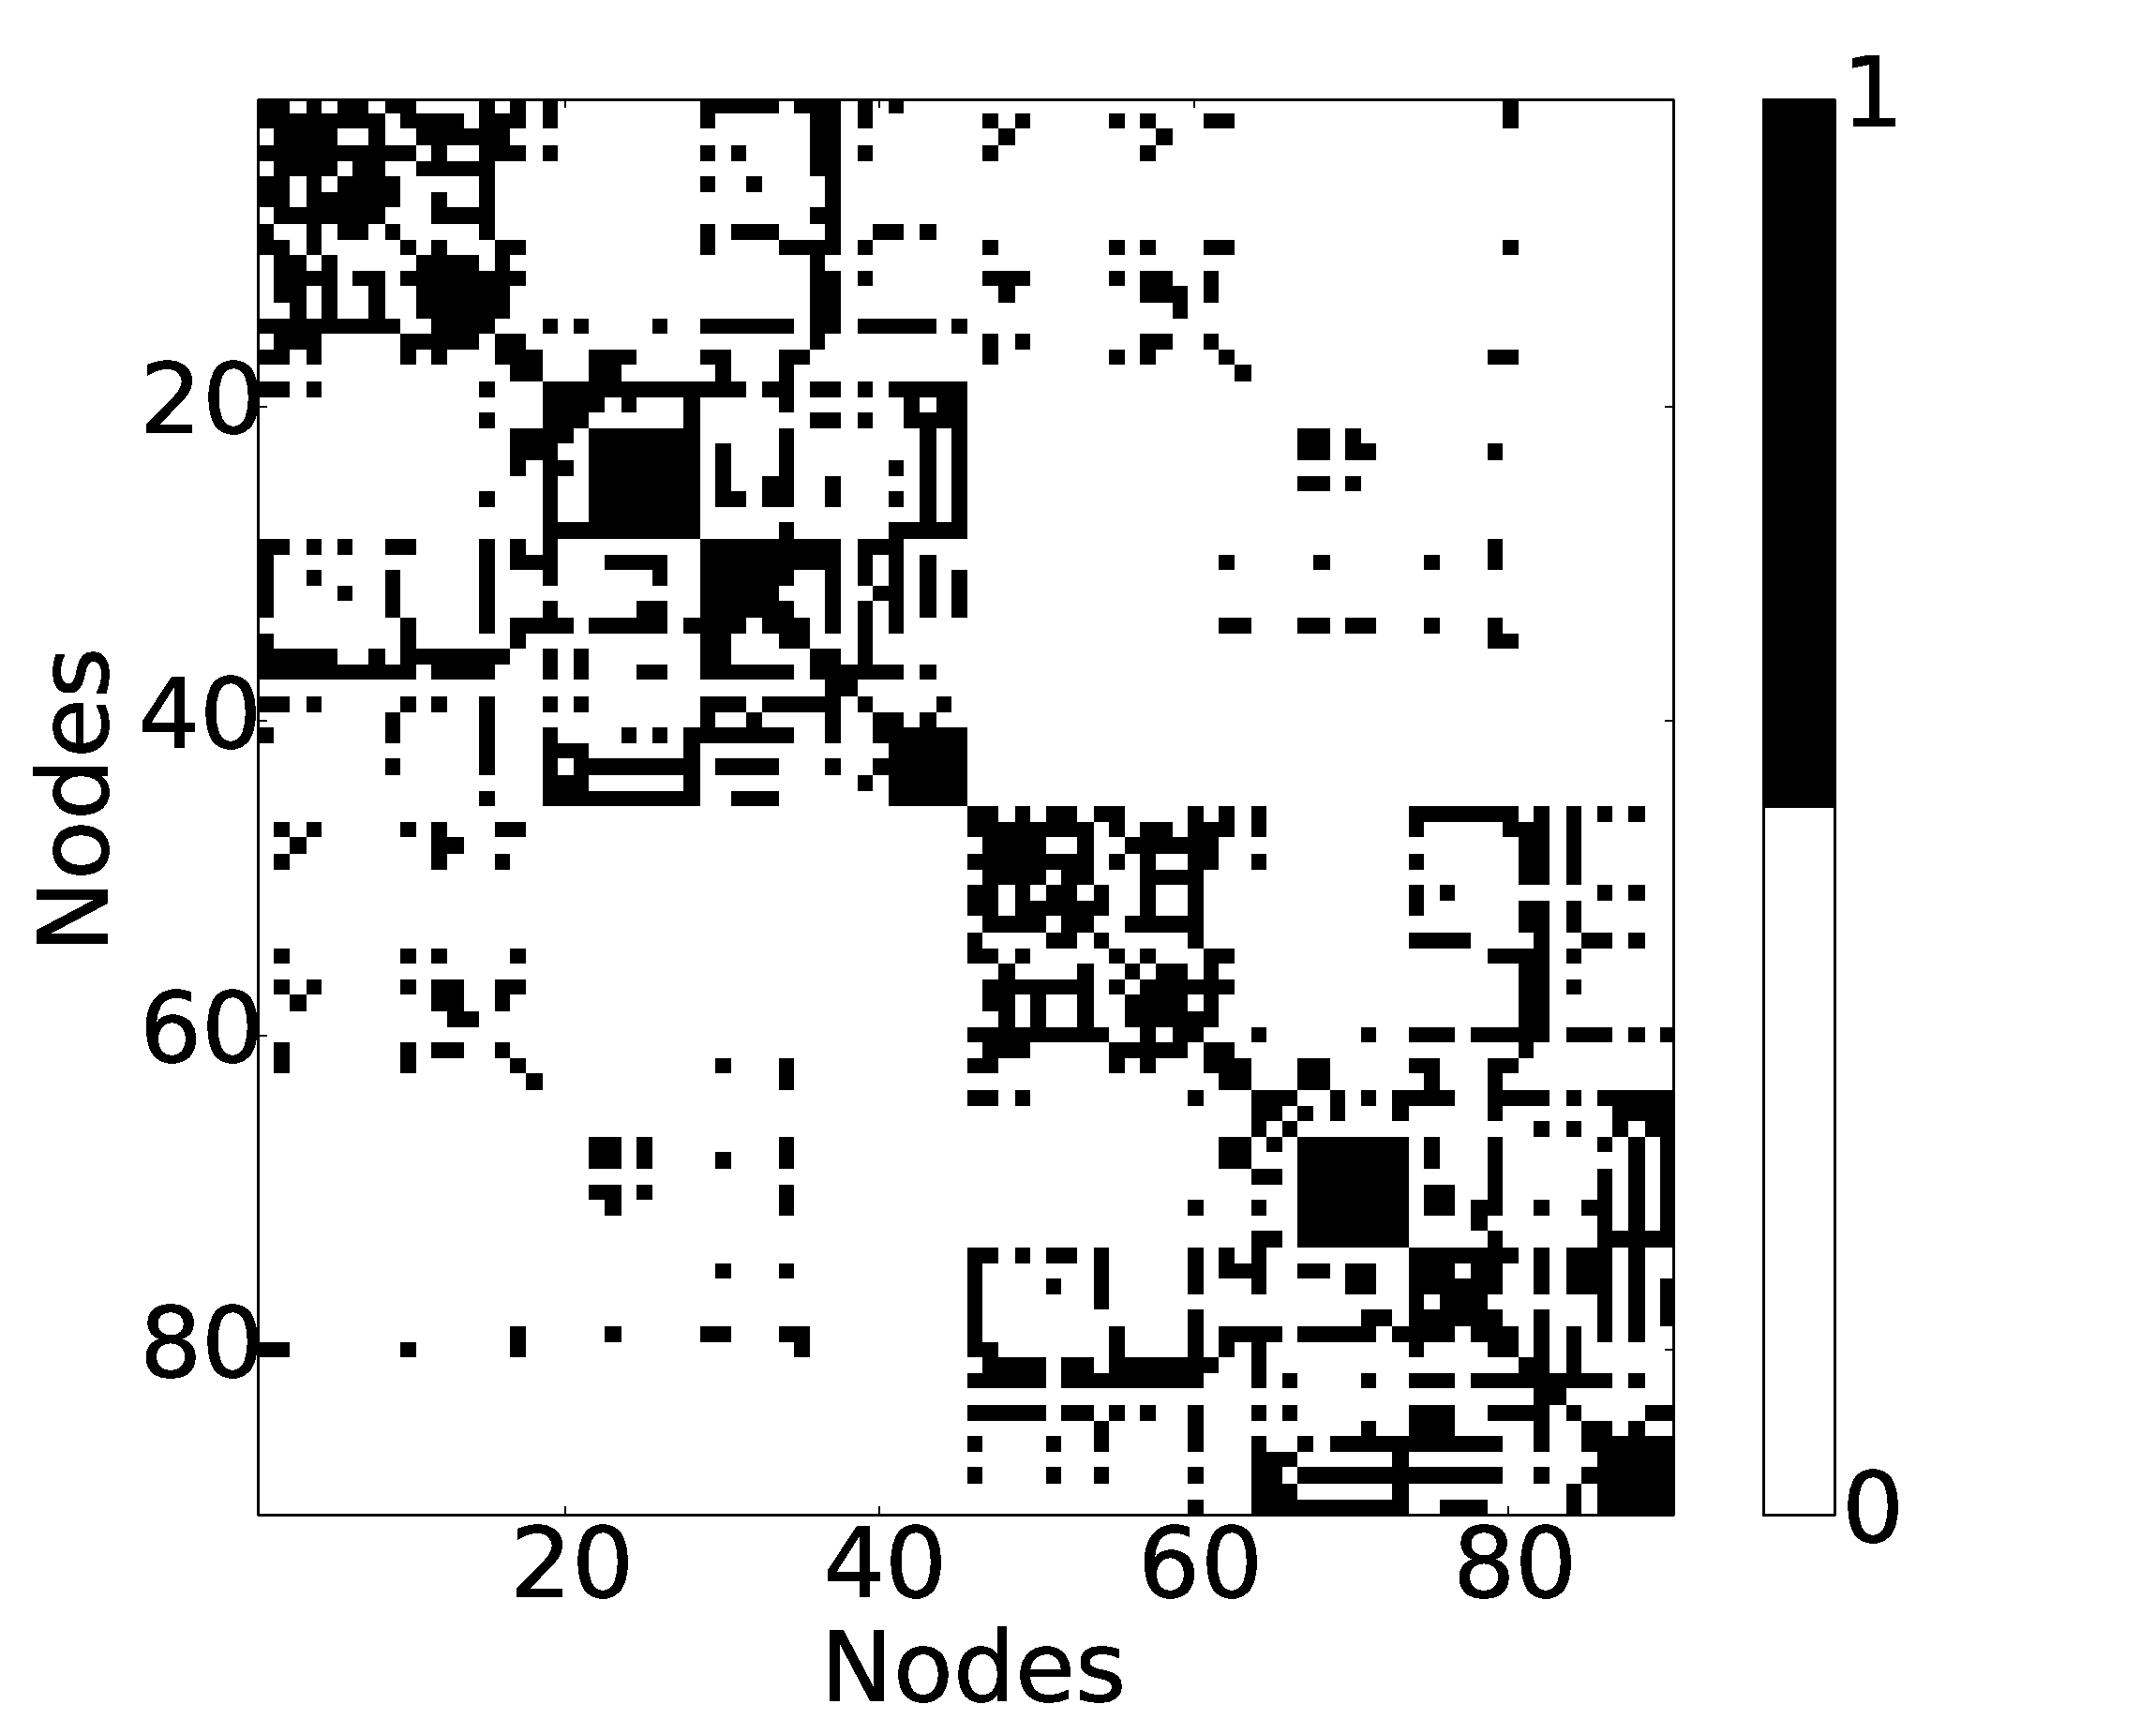
\includegraphics[width=0.49\textwidth]{Figures/Adj_ACM}	 
	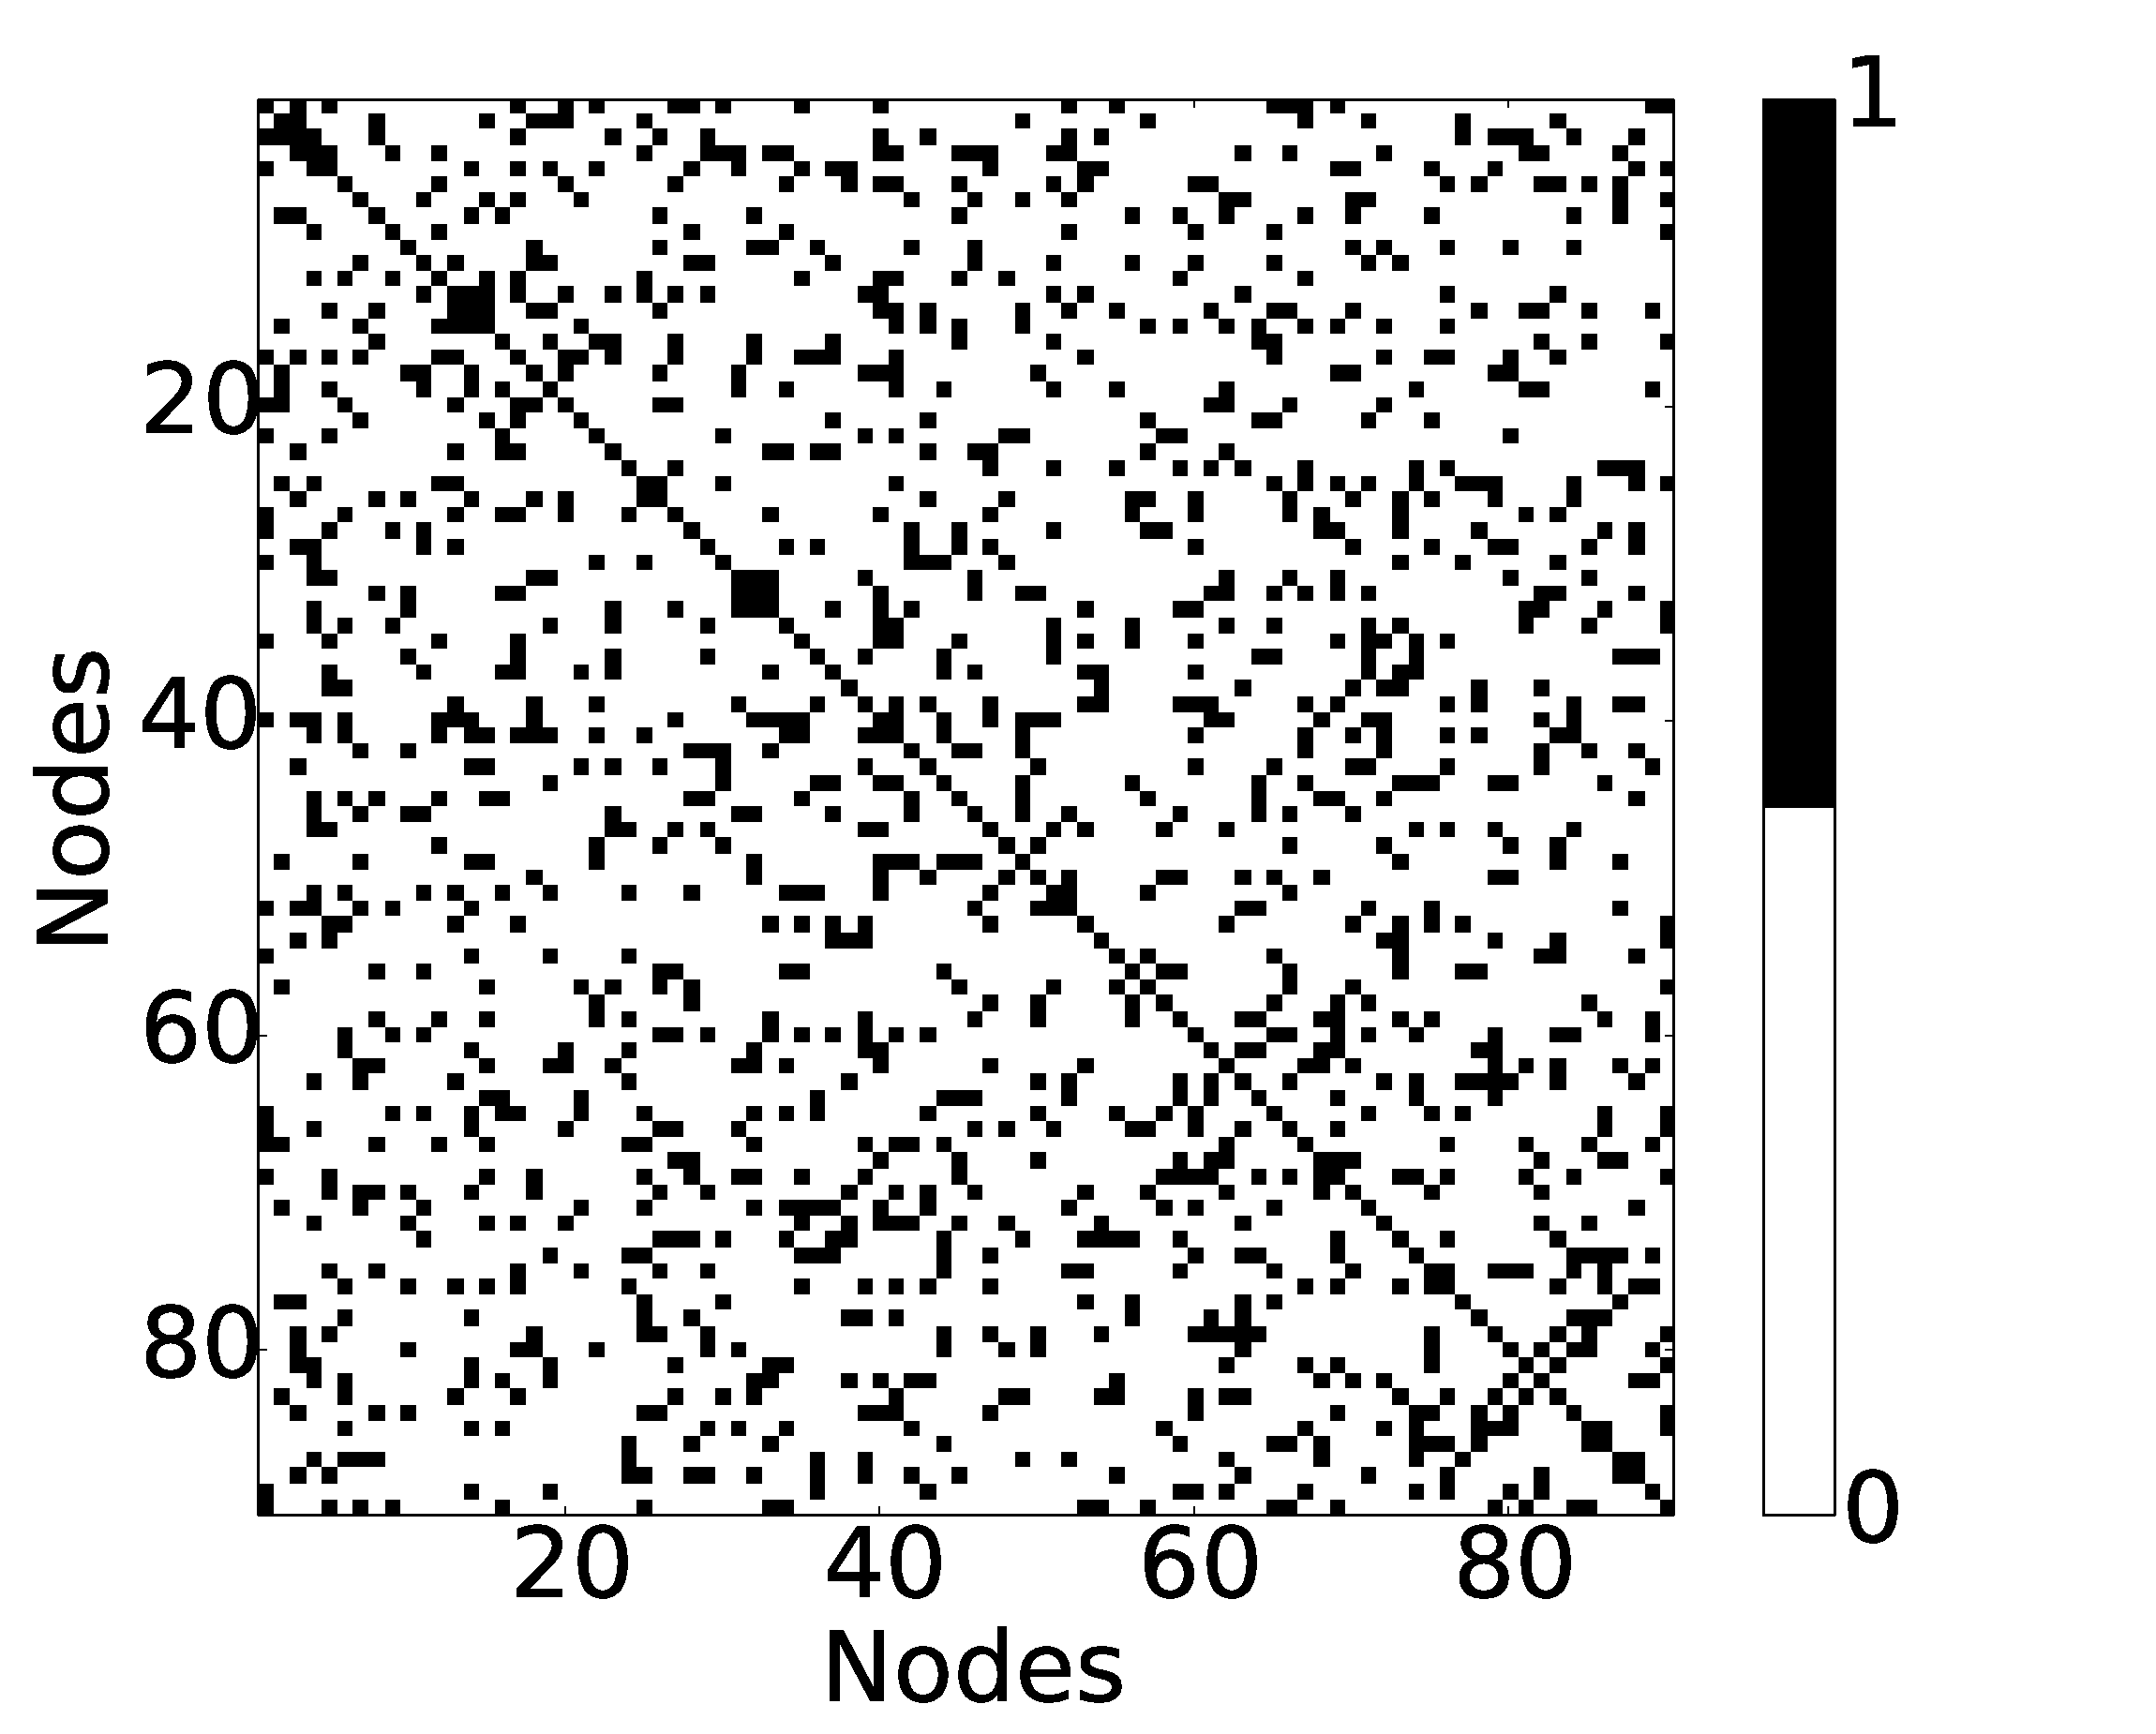
\includegraphics[width=0.49\textwidth]{Figures/Adj_ER} 
\caption{Construction of adjacency matrices: The empirical AC map derived from DW-MRI data is binarized at a
connection probability value $p=0.54$ (left). The black squares represent 1's indicating edges between nodes, whereas
the white squares represent 0's implying no edge. The node index is chosen according to Table~\ref{tab:AAL}. An
Erd\H{o}s-R\'{e}nyi random graph of the same network density is shown in the right panel.}
\label{fig:Binarizing via Thresholding}
\end{figure}

Figure~\ref{fig:Binarizing via Thresholding} illustrates an exemplary construction of adjacency matrices depicting the
empirical connectivity map (left) as well as an Erd\H{o}s-R\'{e}nyi random graph (right). The brain graph is derived
from the AC map seen in Figure~\ref{fig:Empirical FCM and ACM} applying a binarization threshold of $p=0.54$. One can
see
that the nodes of the brain graph are more densely connected within the hemispheres than in the random graph. There is
no specific connection pattern as a result of randomization (right). The network density $\kappa$ is preserved in
the randomized matrix, but the network topology differs. See Appendix for details of network characteristics of $R_{BG}$
and $R_{ER}$.

\subsection*{FitzHugh-Nagumo Model for Neuronal Activity Simulations}
The theoretical model of choice for the neuronal activity is the FitzHugh-Nagumo (FHN) system phenomenologically
describing physiological states of nerve membrane potential \citep{FIT61, NAG62}. The FHN model will be used to
compute the neuronal time series of a nerve cell population, in other words, an AAL node in this study. 

% \paragraph{Local Dynamics}
The local dynamics described by the FHN model consist of an activator variable $x$ and an inhibitor variable $y$.
Following the notation of \cite{GHO08a, GHO08}, it is given by the following nonlinear differential equations:
\begin{subequations}
\begin{align}
  \dot{x} &= \tau \left( y + \gamma x - \frac{x^3}{3} \right)  \label{eqn: frobenius 1}\\  
  \dot{y} &=-\frac{1}{\tau} (x - \alpha + \beta y) , \label{eqn: frobenius 2}   
\end{align} 
\end{subequations}
where $\tau$ denotes the time scale between the fast $x$- and slow $y$-variable, 
% $I$ is the external stimulus parameter
and $\gamma$, $\alpha$, $\beta$ are system parameters. 
$x$ and $y$ are considered to capture the dynamics of a neuronal population.
% be counteracting variables capturing alterations of the membrane potential of a neuronal population of around $10^9$
% cells.
The parameters in the FHN model are chosen such that solutions exhibit a damped oscillatory behavior for each node:
$\alpha = 0.85$, $\beta=0.2$, $\gamma=1.0$, and $\tau=1.25$ \citep{VUK13}. Thus, the fixed point of the system is a
\textit{stable focus}.

% \paragraph{Network Dynamics}
In order to simulate the neuronal activity on the brain graph or random network, the FHN units are coupled as
described by the following set of equations \citep{GHO08, VUK13}:
 \begin{subequations}\label{eq:FHN_network}
 \begin{align}
   \dot{x_i} &= \tau \left( y_i + \gamma x_i - \frac{x_i^3}{3} \right) -c \sum_{j=1}^N a_{ij}x_j\left(t - \Delta 
t_{ij}\right) +Dn_x \label{eqn: frobenius 17}\\  
  \dot{y_i} &= -\frac{1}{\tau} \left(x_i - \alpha + \beta y_i\right) +Dn_y, \label{eqn:frobenius 18} 
\end{align} 
\end{subequations}
where indexes $i, j=1,\dots,N$ represent any node among the $N=90$ AAL regions, $c$ is the coupling strength, which
scales the mutual time-delayed interactions, $\left\{a_{ij}\right\}$ denotes the adjacency matrix obtained at a specific
$p$-value, $n_x$, $n_y$ represent Gaussian white noise sources with zero mean and unity variance and $D$ is the noise
strength. If nodes are connected in a given network, then we have $a_{ij}=1$, otherwise $a_{ij}=0$. $\Delta t_{ij}$ is
the time-delay taking into account a finite signal propagation velocity $v$ between the nodes. $\Delta t_{ij}$ is
calculated as $\Delta t_{ij}=d_{ij}/\nu$ \citep{GHO08, GHO08a, DEC09}, where $d_{ij}$ is the distance matrix for the
approximated fiber lengths between the AAL regions of the AC map \citep{ITU08} (Figure~\ref{fig:d_ij}). We consider a
biophysically realistic velocity of $v=3$m/s \cite{GHO08a}.The noise
strength is fixed at $D=0.05$ throughout this study. The noise variable drives subthreshold oscillations, and the system
does not settle down to the fixed point.

\begin{figure}[t!]
         \centering
	 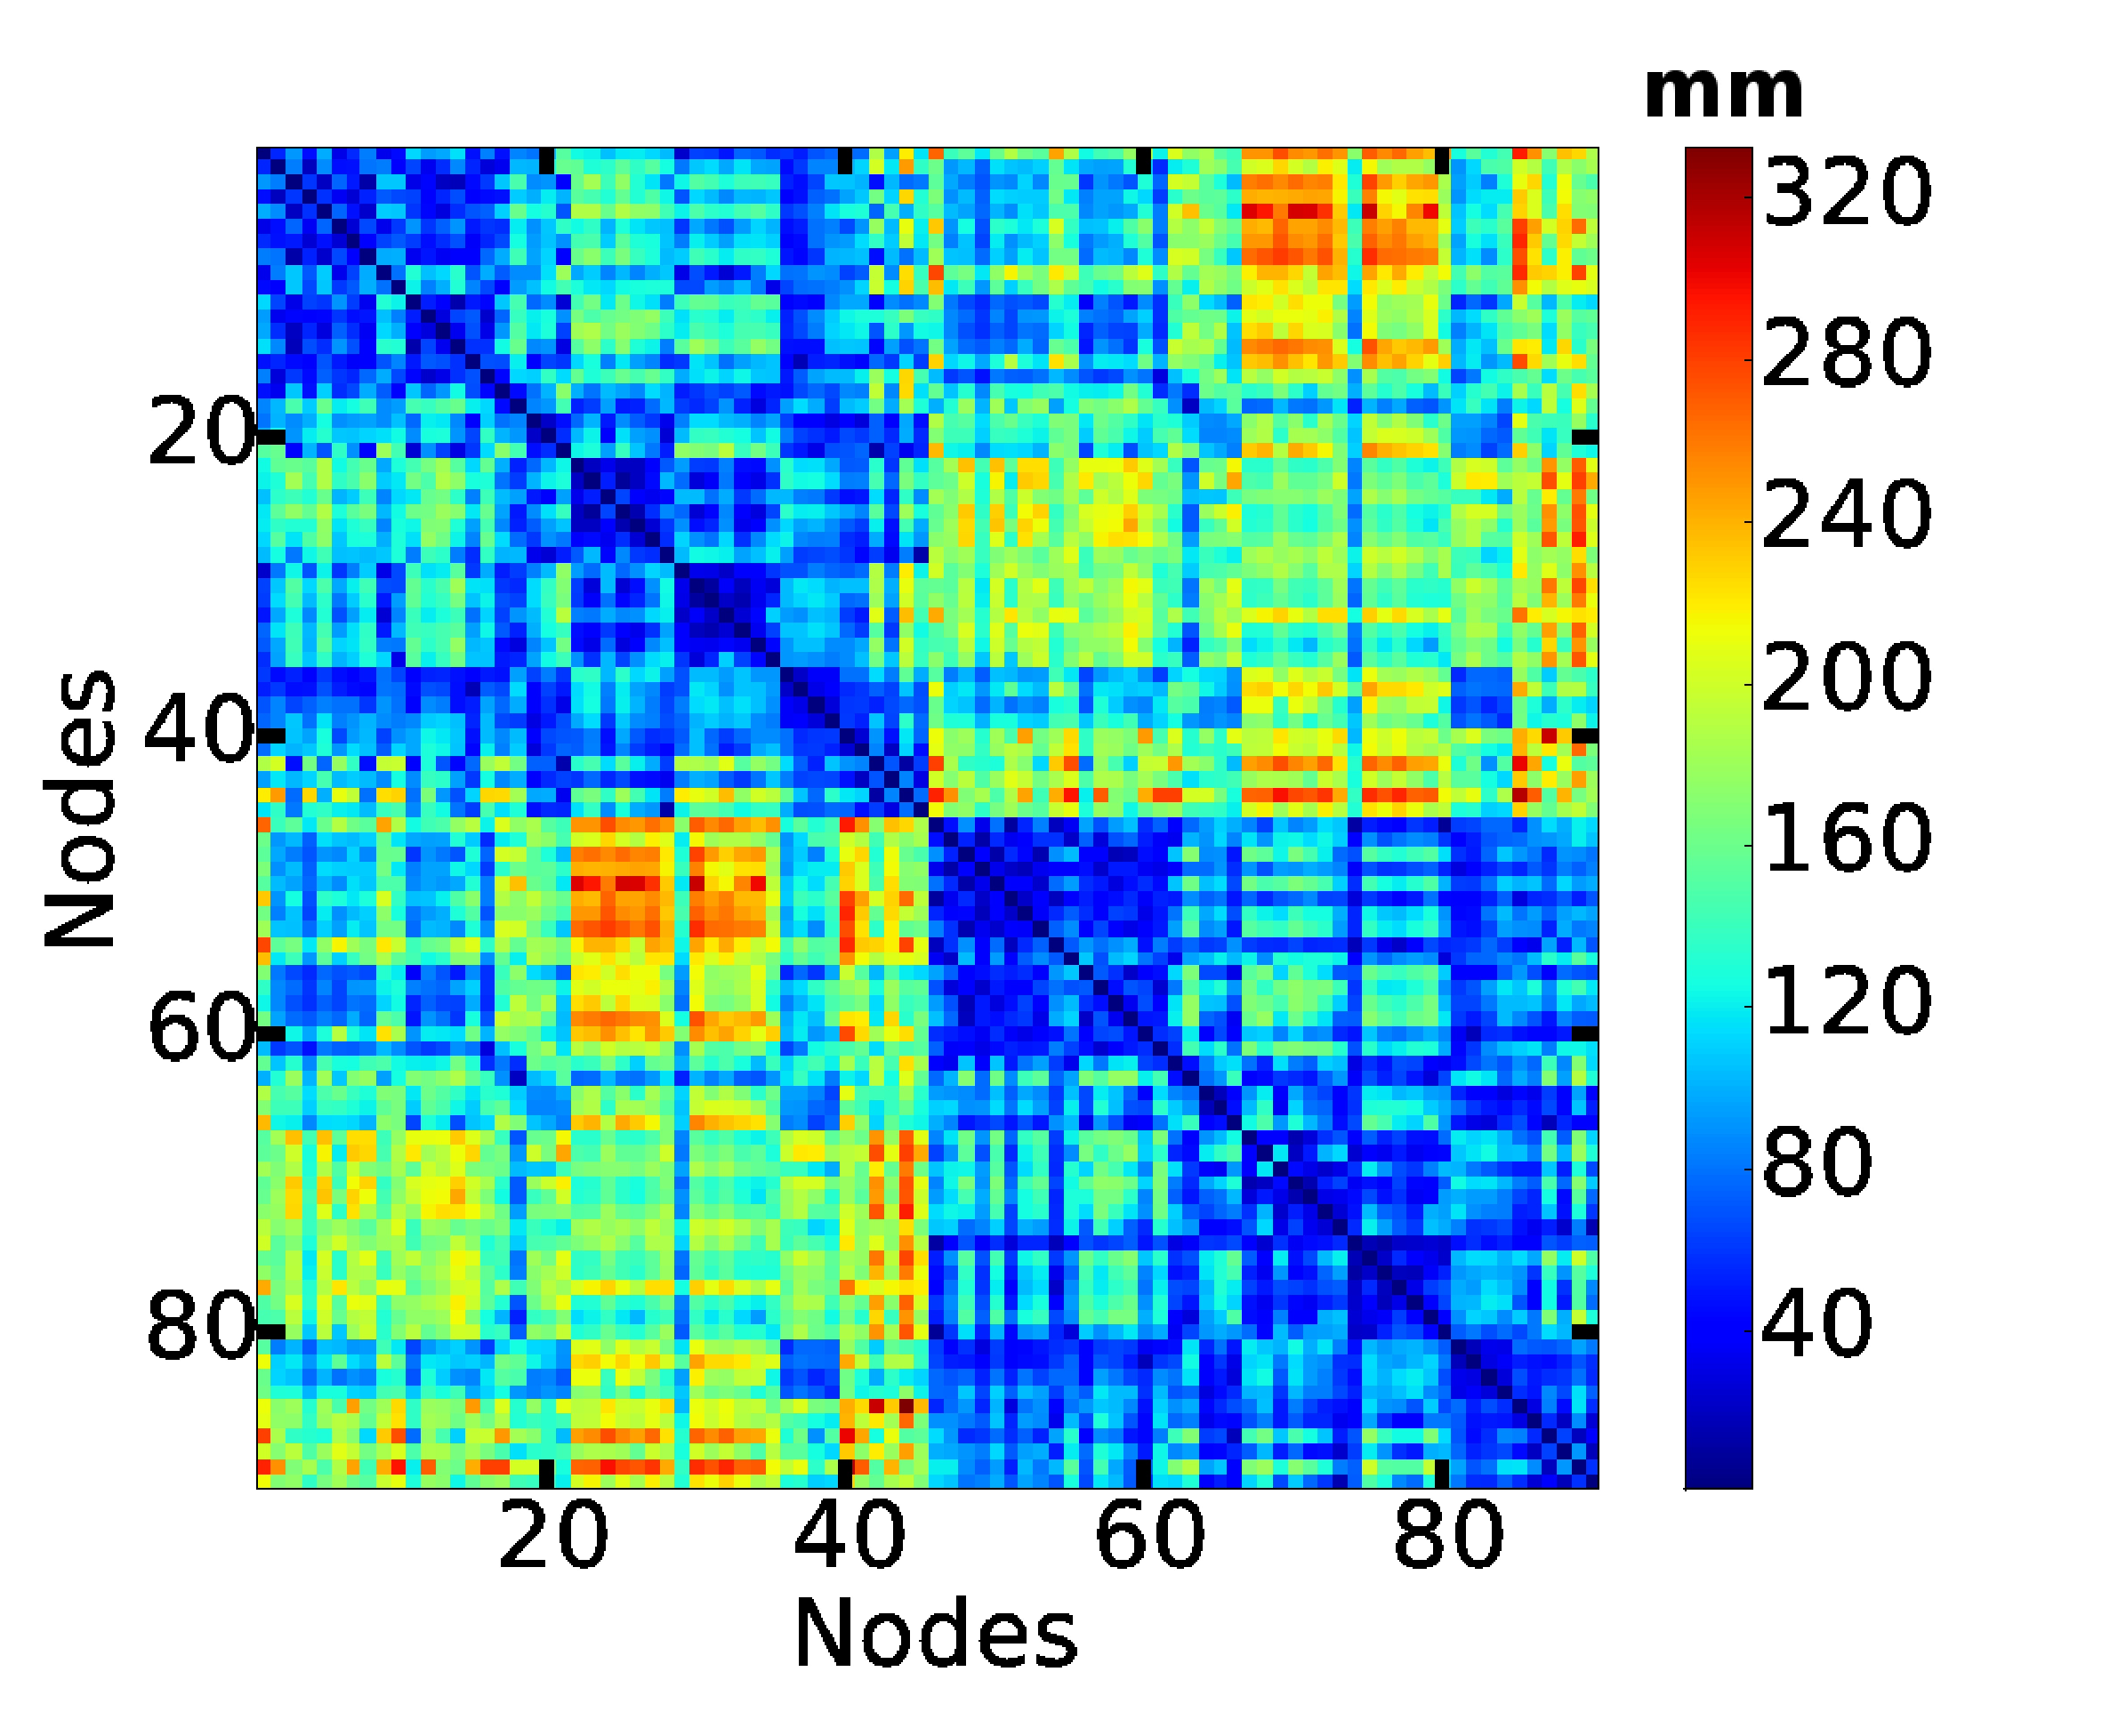
\includegraphics[width=0.49\textwidth]{Figures/distance_ACM_pyt} 
	\caption{Distance matrix $d_{ij}$(mm) given by the fiber length between node pairs.}
\label{fig:d_ij}
\end{figure}

The  set of delay differential equations~(\ref{eq:FHN_network}) is solved numerically using the \textsc{PYTHON}-module
\textsc{PYDELAY} (\textit{http://pydelay.sourceforge.net}) based on Bogacki-Shampine method \citep{BOG89,
FLU09a}. We simulate 7.5 minutes of neuronal activity, which corresponds to the length of the empirical BOLD
measurement and we discard transients of 20 s.

\subsection*{Balloon-Windkessel Model for BOLD Activity Simulations} 
From the simulated neuronal activity, we infer the BOLD signal observed in the fMRI data via the
Balloon-Windkessel hemodynamic process
% , which mediates between neuronal activity and its  BOLD response 
\citep{FRI00}.
In short, the Balloon-Windkessel model uses the neuronal time series as an input signal  \citep{SET12}and computes
hemodynamic oscillations analogous to the BOLD signal, which is modeled as a function of changes in cerebral blood flow,
cerebral blood volume and cerebral metabolic rate of oxygen consumption. 
% The main input of the Baloon-Windkessel model is a neuronal signal in the form of either a spiking rate or a local field
% potential. 
The neuronal signal in the current study will be the normalized time series of the activator variables.
% , which describes
% the excitatory membrane potential dynamics of a neuronal population. 
Friston et al. have shown that it is possible to capture ultra-slow frequency oscillations ($<0.1$ Hz) in the
hemodynamic process, given high-frequency neuronal input \citep{FRI00}. Here, the same
model will be used for the  resting-state activity 
% to find out whether it is possible to extract BOLD activity from
% FHN-modeled 
of the $N=90$ AAL brain regions.

\subsection*{Comparing Simulated and Empirical Correlation Matrices}       
One of the research proposals of this paper is to investigate whether FC in human brain at
rest can be computed from AC based a self-organized dynamical process. To answer this
question, the brain graphs obtained from AC maps are used in the simulation to compute functional correlations based
on the BOLD activity. These correlations of simulated BOLD activity between any node pairs $i,j$ are quantified by
the Pearson's correlation coefficient $\rho_{i,j}$, 
\begin{equation}
\rho_{i,j} = \dfrac{\big \langle u_i(t) u_{j}(t) \big \rangle - \big \langle u_{i}(t) \big \rangle  \big \langle
u_{j}(t) \big \rangle}{ \sigma (u_i(t)) \sigma (u_j(t))},
\end{equation}
where $u_i(t)$ denotes the BOLD time series of the node $i$,  $\sigma$ stands for standard deviation and
$\big \langle \cdot \big \rangle$ represents the temporal average. 
% Then, the results are compared statistically to the empirical FC
% map. 
% All $\rho_{i,j}$ values among any possible pairwise combination of $N=90$ nodes are then used to built a $90\times 90$ 
% matrix, which is referred to as simulated functional connectivity (FC$_s$). 
This yields a $90\times 90$ correlation matrix  $\left\{\rho_{i,j}\right\}$, which is referred to as simulated
functional connectivity (FC$_s$).
In order to compare our modeling approach to the empirical result, the FC$_s$ and the empirical FC map (FC$_e$)
-- derived from fMRI-BOLD measurements -- are compared statistically with Pearson's correlation coefficient $\rho_{e,s}$
in dependence on the binarization threshold $p$ and coupling strength $c$.
% , the same linear pairwise correlation method again.
% All correlation values $\rho_{e,s}$ between empirical $e$ and
% simulated $s$ data matrices will
% be placed in the parameter space $(p,c)$. 


\subsection*{Comparing Brain Graphs to Random Graphs}

The topological properties of the brain graph $R_{BG}$ and random graph $R_{ER}$ are illustrated  in
Figure~\ref{fig:network measures}. Note that the network density $\kappa$, \textit{average clustering coefficients} $C$,
and \textit{small-worldness} $S$ of each network are calculated and visualized in dependence on the binarization
threshold $p$. For formal definitions of $C$ and $S$, see Appendix. Figure~\ref{fig:network measures}
(left) shows that $\kappa$ of $R_{BG}$ is preserved in $R_{ER}$, as expected from the definition of
Erd\H{o}s-R\'{e}nyi-type randomization. $\kappa$ decreases sigmoidally with increasing $p$. Figure~\ref{fig:network
measures} (middle) indicates that $R_{BG}$ has a higher clustering coefficient $C$ compared to $R_{ER}$, meaning
that nodes in $R_{BG}$ tend to cluster more. Therefore, the local information transfer is expected to be more efficient
in $R_{BG}$. The networks are also clearly distinguishable in terms of $S$-values as seen in Figure~\ref{fig:network
measures} (right). The brain graph appears to be more segregated (local clusters) and integrated (existence of
shortcuts) than corresponding random graphs of the same network density.


\begin{figure}[t!]
\centering
	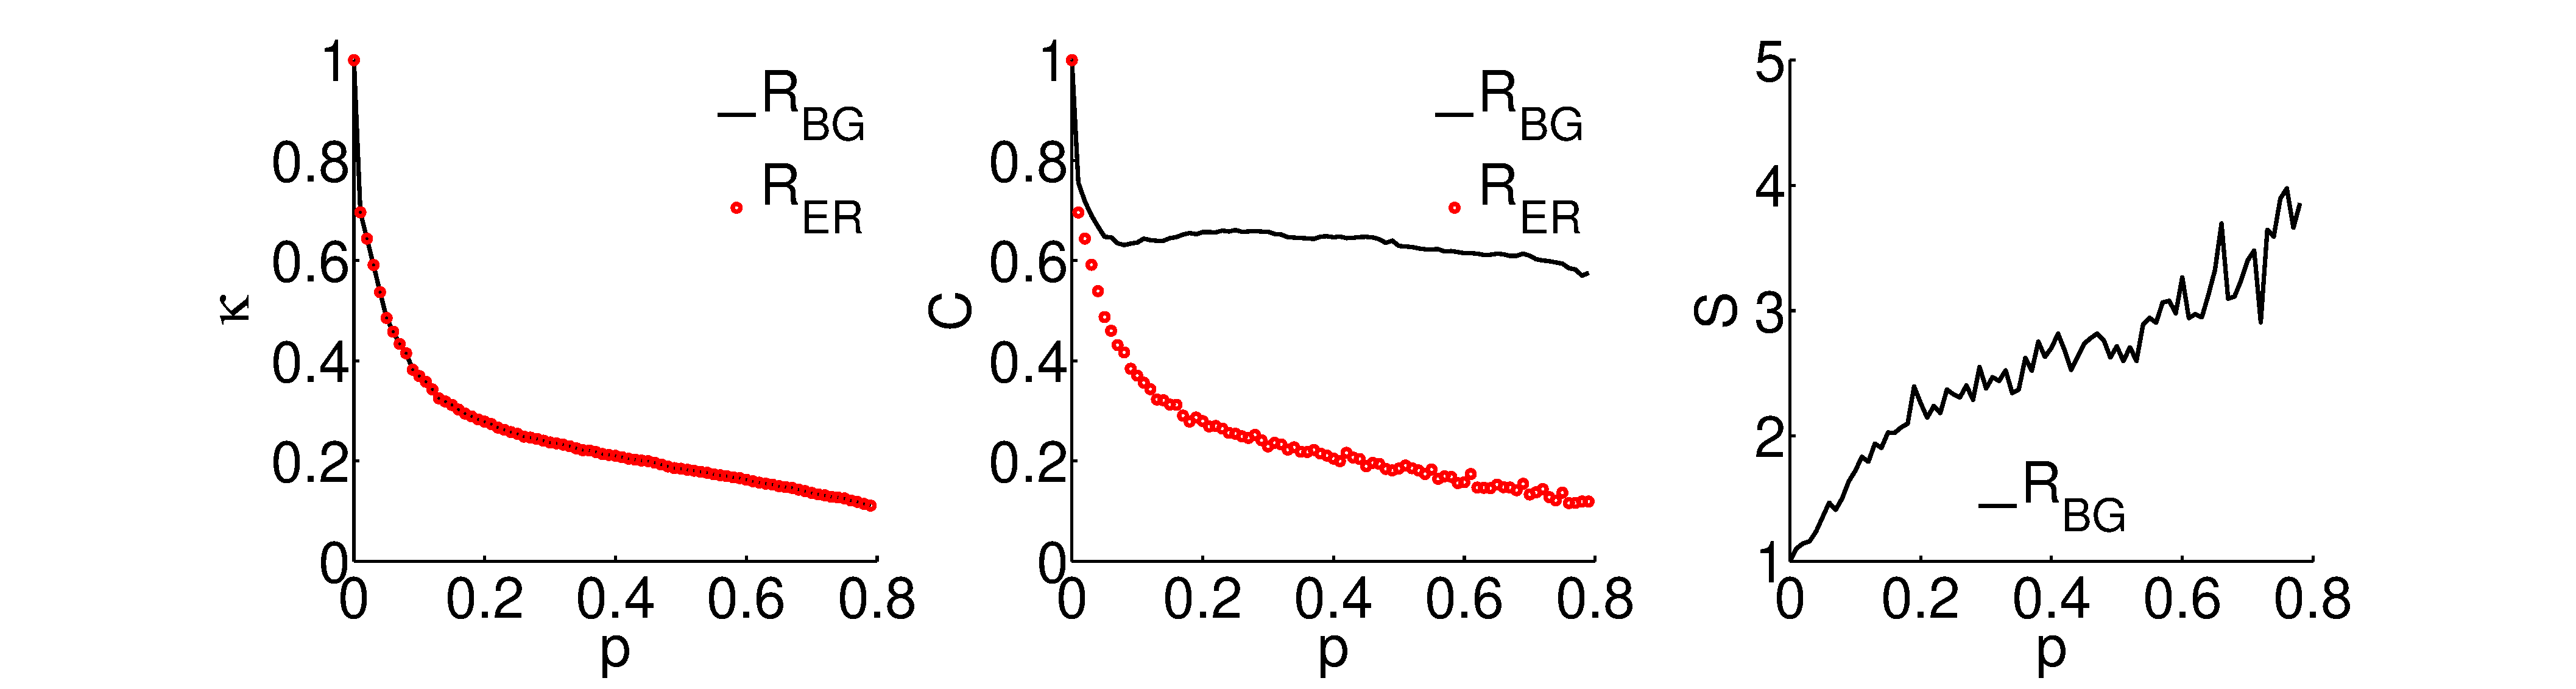
\includegraphics[width=\textwidth]{Figures/network_meas_05}  
\caption{Statistical network characteristics of $R_{BG}$ (black curves) and $R_{ER}$ (red dots): Network density
$\kappa$ (left), cluster coefficient $C$ (center) and small-worldness coefficient $S$ (right). $S$ is only shown in the
range, where the network is connected.\\
%%\red{Remove green lines, reduced x-range to [0,0.79] (right panel), add ticks and labels for 0, 0.2, 0.4, 0.6, 0.8 on
%all axes.}
}
\label{fig:network measures}
\end{figure}


In addition, we compare the brain graph $R_{BG}$ and random graph $R_{ER}$ not only in terms of several
network measures, but also their modeled temporal dynamics, which is obtained from FHN network model and BOLD activity
simulations. 
% The
% Pearson correlation coefficients $\rho$
% between any pairwise combinations of $N=90$ nodes are calculated for their modeled time series in each network. These
% correlation coefficients are then distributed in histograms at $(p,c)$-values. 
To quantify the similarity of modeled temporal activity on $R_{BG}$ and $R_{ER}$, we calculate
Bhattacharya coefficients of the histograms of the simulated correlation matrices, a widely used
statistical approach to measure the correlation between statistical samples as detailed in the following \citep{XYZ43}.

Let us denote the histogram of simulated correlation $\rho_{i,j}$ of $R_{BG}$ by $H_{BG}$ and that of
$R_{ER}$ by $H_{ER}$. Then, the Bhattacharya coefficient $d\left(H_{BG}, H_{ER}\right)$ is given by the following
equation:
\begin{equation}
d\left(H_{BG}, H_{ER}\right) = \sqrt{1- \dfrac{1}{ \sqrt{\overline{H}_{BG}\, \overline{H}_{ER} N^2}} \sum_{i}
\sqrt{H_{BG}(i)H_{ER}(i)} } ,
\end{equation}
where $\overline{H}$ denotes the mean of the histogram $H$ \citep{XYZ43}. $d\left(H_{BG}, H_{ER}\right)$ is scaled
between 0 and 1. A high $d\left(H_{BG}, H_{ER}\right)$ value indicates a small overlap of $H_{BG}$ and $H_{ER}$,
whereas a low $d\left(H_{BG}, H_{ER}\right)$ value expresses a high degree of similarity. 

% \reg{PH: CONTINUE FROM HERE}

\section*{Results \& Discussion}
% \subsection*{Network Measures of Brain Graph vs Random Graph}

% \newpage
% \subsection*{Modeled BOLD Activity on Anatomical Connectivity Map}
For each combination of threshold $p$ and coupling strength $c$, we calculate a simulated functional
connectivity matrix FC$_s$ from the numerical BOLD signal. The FC$_s$ and empirically derived functional connectivity
matrix FC$_e$ (Figure~\ref{fig:Empirical FCM and ACM}, left) are
compared quantitatively by Pearson's correlation coefficients $\rho_{e,s}$ in parameter space $(p,c)$.
% The results
% are shown in Figure~\ref{fig:PA_p_c}.

% We investigated that it would be possible to capture functional activity at resting-state through the anatomical
% connectivity in human brain. 

\begin{figure}[t!]
\centering
	\includegraphics[width=0.57\textwidth]{Figures/PA_ACM_BOLD_v_3_new_01}  
\caption{Parameter analysis for the statistical comparison of FC$_e$ and FC$_s$ in the $(p,c)$-space. Parameters:
$\alpha = 0.85$, $\beta=0.2$, $\gamma=1.0$, $\tau=1.25$, and $v=3$~m/s.\\
%\red{Reduce the number of tick labels. Keep only 0.01, 0.02 etc. Remove the row for $c=0.1$ because of the jump from
%0.05 to 0.1.}
% The FC$_e$ is
% unique and refers to the FC map in Figure~\ref{fig:Empirical FCM and ACM} (left). Several FC$_s$ matrices are obtained
% via modeling BOLD temporal dynamics on the AC map, which is shown in Figure~\ref{fig:Empirical FCM and ACM} (right).
% The
% colorbar represents $\rho_{e,s}$ between empirical and simulated matrices. The results are exhibited for weekly coupled
% functional interactions with low $c$-values. $p$-values are considered to be between 0.18 and 0.82 by increment of 0.04.
% The signal propagation velocity $v$ is fixed as 3 m/s.
}
\label{fig:PA_p_c}
\end{figure}

Figure~\ref{fig:PA_p_c} shows that the statistical match between simulated and empirical BOLD activity correlations tend
to be high at relatively low coupling strengths $c \leq 0.1$ and connection probability $0.34 <p<0.70$ as visualized by
hot colors. This range of $p$-values corresponds to a network density $0.23 \geq \kappa \geq 0.17$ (cf.
Figure~\ref{fig:network measures}), which is in agreement \cite{BUL11}. 
% We find the best agree ment between simulated and empirical FC for $c=0.03$ and $p=0.54$.
% In particular, it can be inferred that, the smaller
% scaled the neuronal activity oscillations are, the
% higher correlation between FC$_s$ and FC$_e$ is captured. 
%  It should be also mentioned that the signal propagation velocity $v$ is
% fixed to 3 m/s, which corresponds to the lower boundary for a biophysically plausible signal velocity range
% \citep{GHO08}. 

\begin{figure}[htpb]\centering
	 \includegraphics[width=0.49\textwidth]{Figures/cor_BOLD_ACM_sim} 
%   	 \includegraphics[width=0.49\textwidth]{Figures/cor_FCM_exp} 
  \caption{Simulated functional connectivity matrix FC$_s$ for a threshold $p=0.54$ and coupling
strength $c=0.03$ corresponding to $\rho_{e,s} = 0.22$.
% Modeling parameters are $p=0.54$ and $c=0.03$. 
Other parameters as in Figure~\ref{fig:PA_p_c}.} 
    \label{fig:BOLD_e_s}
\end{figure}  

We find the best agreement between FC$_s$ and FC$_e$ at $c=0.03$ and $p=0.54$ ($\rho_{e,s}=0.22$).
Figure~\ref{fig:BOLD_e_s} depicts the FC$_s$ matrix at these particular parameter values. Here, the colorbar denotes the
pairwise Pearson's coefficients $\rho_{i,j}$ between the modeled BOLD time series of all
possible node pairs ${i,j}$. In comparison to the FC$_e$ in Figure~\ref{fig:Empirical FCM and ACM} (left), FC$_s$ tends
to reproduce some clusters of well correlated regions along the main diagonal, but it does not show pronounced
functional correlation of corresponding brain regions in the two hemispheres. Only a few inter-hemispheric correlations
are visible. Furthermore, the intra-hemispheric correlations within the right hemisphere (bottom right quadrant) are in
agreement with the empirical observation $\rho_{e,s}(RR)=0.52$, where as the simulation does not show strong correlation
with the left hemisphere ($\rho_{e,s}(LL)=0.40$). We attribute this difference from the empirical measurement to
asymmetries with respect to the two hemispheres and to longer time delays in the left hemisphere (cf.
Figure~\ref{fig:d_ij}).

% Top left quadrants (nodes in left hemisphere $i,j=\{1,2,...,45\}$)
% and bottom right quadrants (nodes in right hemisphere $i,j=\{46,47,...,90\}$) in both matrices correlate with higher
% Pearson coefficients: $\rho_{e,s}(LL)=0.40$ and . The FC$_s$ does not exhibit high correlating
% inter-hemispheric nodes as dominant as in FC$_e$. The longer distances between right and left hemispheric nodes might be
% the reason, why our model cannot successfully reproduce the inter-hemispheric correlations (see Figure~\ref{fig:d_ij}). 

\begin{figure}[htpb] \centering
	 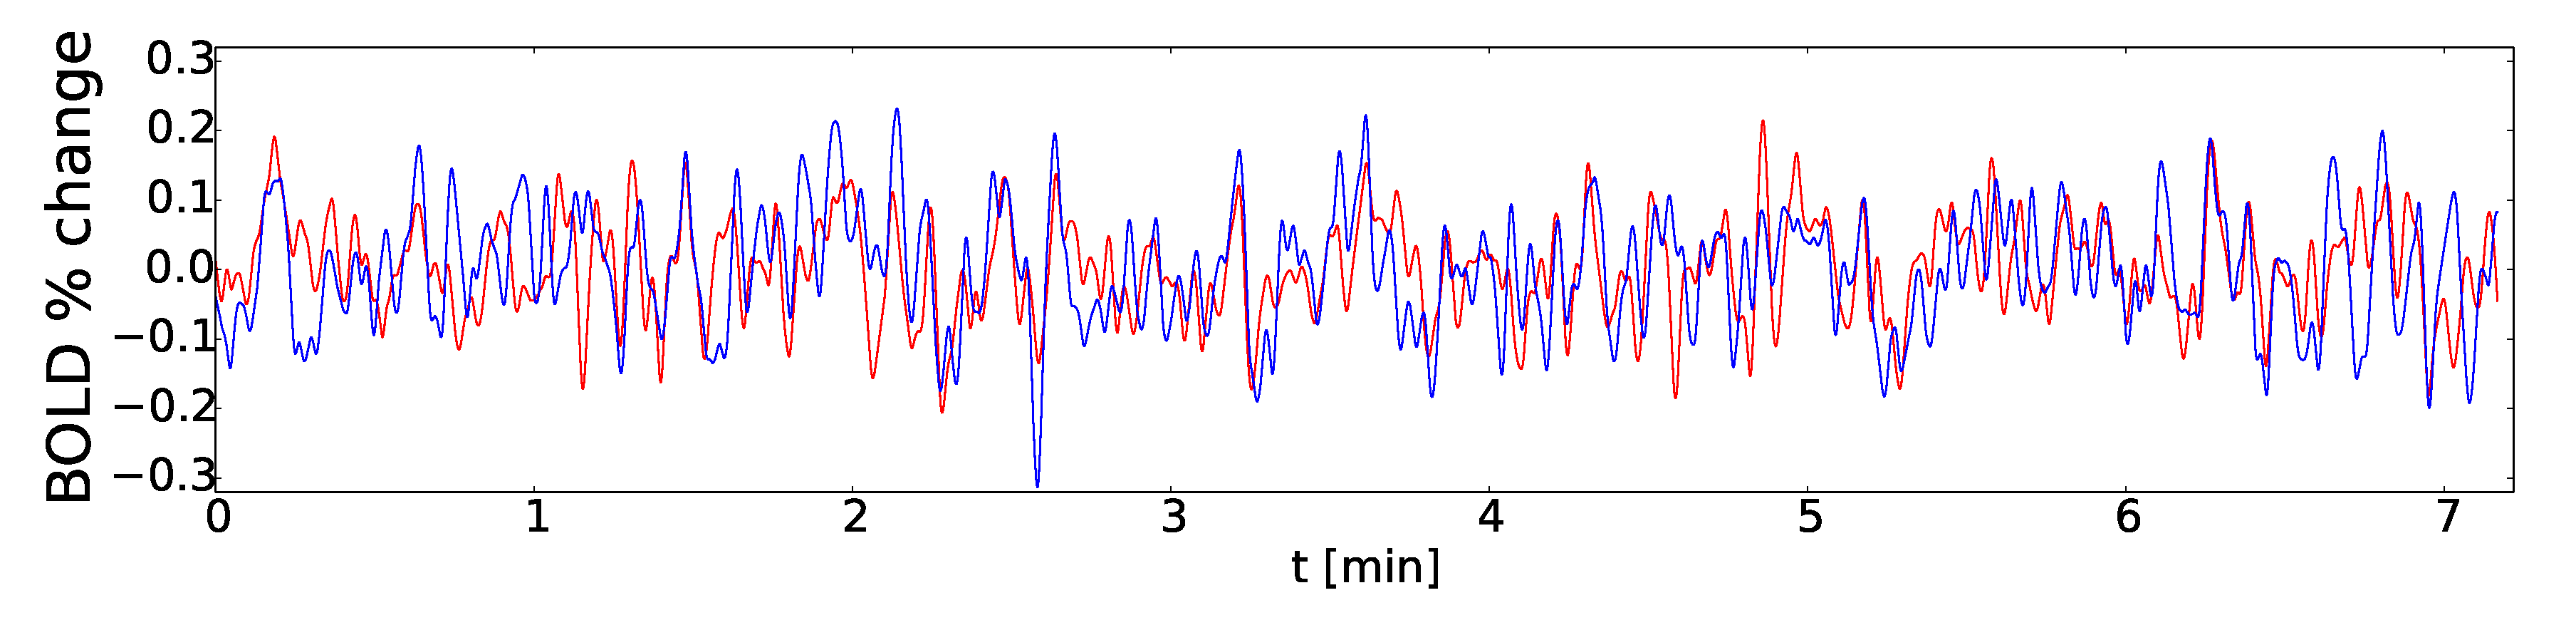
\includegraphics[width=\textwidth]{Figures/cor_BOLD_ACM_sim_no_best_new} 
   \caption{Simulated BOLD activity of highly correlated node pairs (red: $u_{58}$, blue: $u_{59}$) with
$\rho_{58,59}=0.48$. A transient of 20s was discarded.
% Both nodes are chosen from the FC$_s$ in Figure~\ref{fig:BOLD_e_s} 
Parameters as in Fig~\ref{fig:BOLD_e_s}.
% ($c=0.03$, $v=3$ m/s, $p=0.54$).
} 
  \label{fig:BOLD_nodes}
\end{figure} 

Starting from fast oscillating neuronal time series as the input, the Balloon-Windkessel hemodynamic model acts as a
low-pass filter \citep{FRI00}. The resulting BOLD fluctuations are ultra slow in the frequency range below 0.1 Hz and,
we find the BOLD activity of our simulations to be in this plausible frequency domain. Figure~\ref{fig:BOLD_nodes}
depicts the temporal dynamics of the simulated BOLD activity of a node pair. This node couple shows pronounced FC$_s$ in
Figure~\ref{fig:BOLD_e_s}. The extracted BOLD oscillations of nodes 58 (L, Frontal Mid Orb) and 59 (L, Gyrus Rectus) are
correlated with $\rho_{58,59}=0.48$. 

% \subsection*{Temporal Dynamics of Brain Graph vs Random Graph}   
The AC map is binarized at probability values in $0.34 \leq p \leq 0.82$ range by amount of 0.04 step size.
% $R_{BG}$ and
% $R_{ER}$ is constructed at each $p$-value, then the neuronal activity as well as the BOLD fluctuations are modeled on
% each network. 
Figure~\ref{fig:BG_vs_RG_v_3} compares the simulated temporal dynamics on the brain graph $R_{BG}$ and random graph
$R_{ER}$; for the FHN network model (left) and the Balloon-Windkessel model (right) in the parameter space $(p,c)$.
These comparisons are quantified by Bhattacharya coefficients $d(H_{BG}, H_{ER})$ given by color bars, where $H_{BG}$
and
$H_{ER}$ refer to histogram of the FC matrices of simulations on $R_{BG}$ and $R_{ER}$, respectively. 
% Here, the
% $H_{BG}$ and $H_{ER}$ are obtained by calculating $\rho_{i,j}$-values for
% the simulated time series at specific $(p,c)$-values (see Figure~\ref{fig:histo_ex}). 

In Figure~\ref{fig:BG_vs_RG_v_3}, the hot colors indicate a difference between $H_{BG}$ and $H_{ER}$, whereas the cold
colors refer to similar histograms. The FC based on the neuronal time series modeled by the FHN equations on network
$R_{BG}$ can be clearly distinguished from that of $R_{ER}$
% at $0.34 \leq p \leq 0.78 $ and at $0.015\leq c \leq 0.035$ 
See Figure~\ref{fig:BG_vs_RG_v_3} (left). Only for very weak or strong coupling $d(H_{BG}, H_{ER})$ is small and thus, the
histograms similar. However, a clear pattern of diversity cannot be captured for the BOLD activity
simulations between $R_{BG}$ and $R_{ER}$ (right).  

\begin{figure}[ht] \centering
	 \includegraphics[width=0.48\textwidth]{Figures/Random_ACM_PA_task_v_3_FHN_01} 
	 \includegraphics[width=0.48\textwidth]{Figures/Random_ACM_PA_task_v_3_BOLD_01} 
   	 \caption{Statistical comparison of brain graphs $R_{BG}$ and random graphs $R_{ER}$ in terms of their
modeled temporal dynamics: FHN network model (left) and modeled BOLD activity (right). The heat map represents the
degree of similarity $d\left(H_{BG}, H_{ER}\right)$ between histogram distributions of simulated functional connectivity
of $R_{BG}$ and $R_{ER}$. Parameters as in Fig~\ref{fig:PA_p_c}.\\
%\red{Do we have the values for larger $c$ as in Fig.~\ref{fig:BG_vs_RG}?}
} 
    \label{fig:BG_vs_RG_v_3}
\end{figure}

\begin{figure}[ht] \centering
	 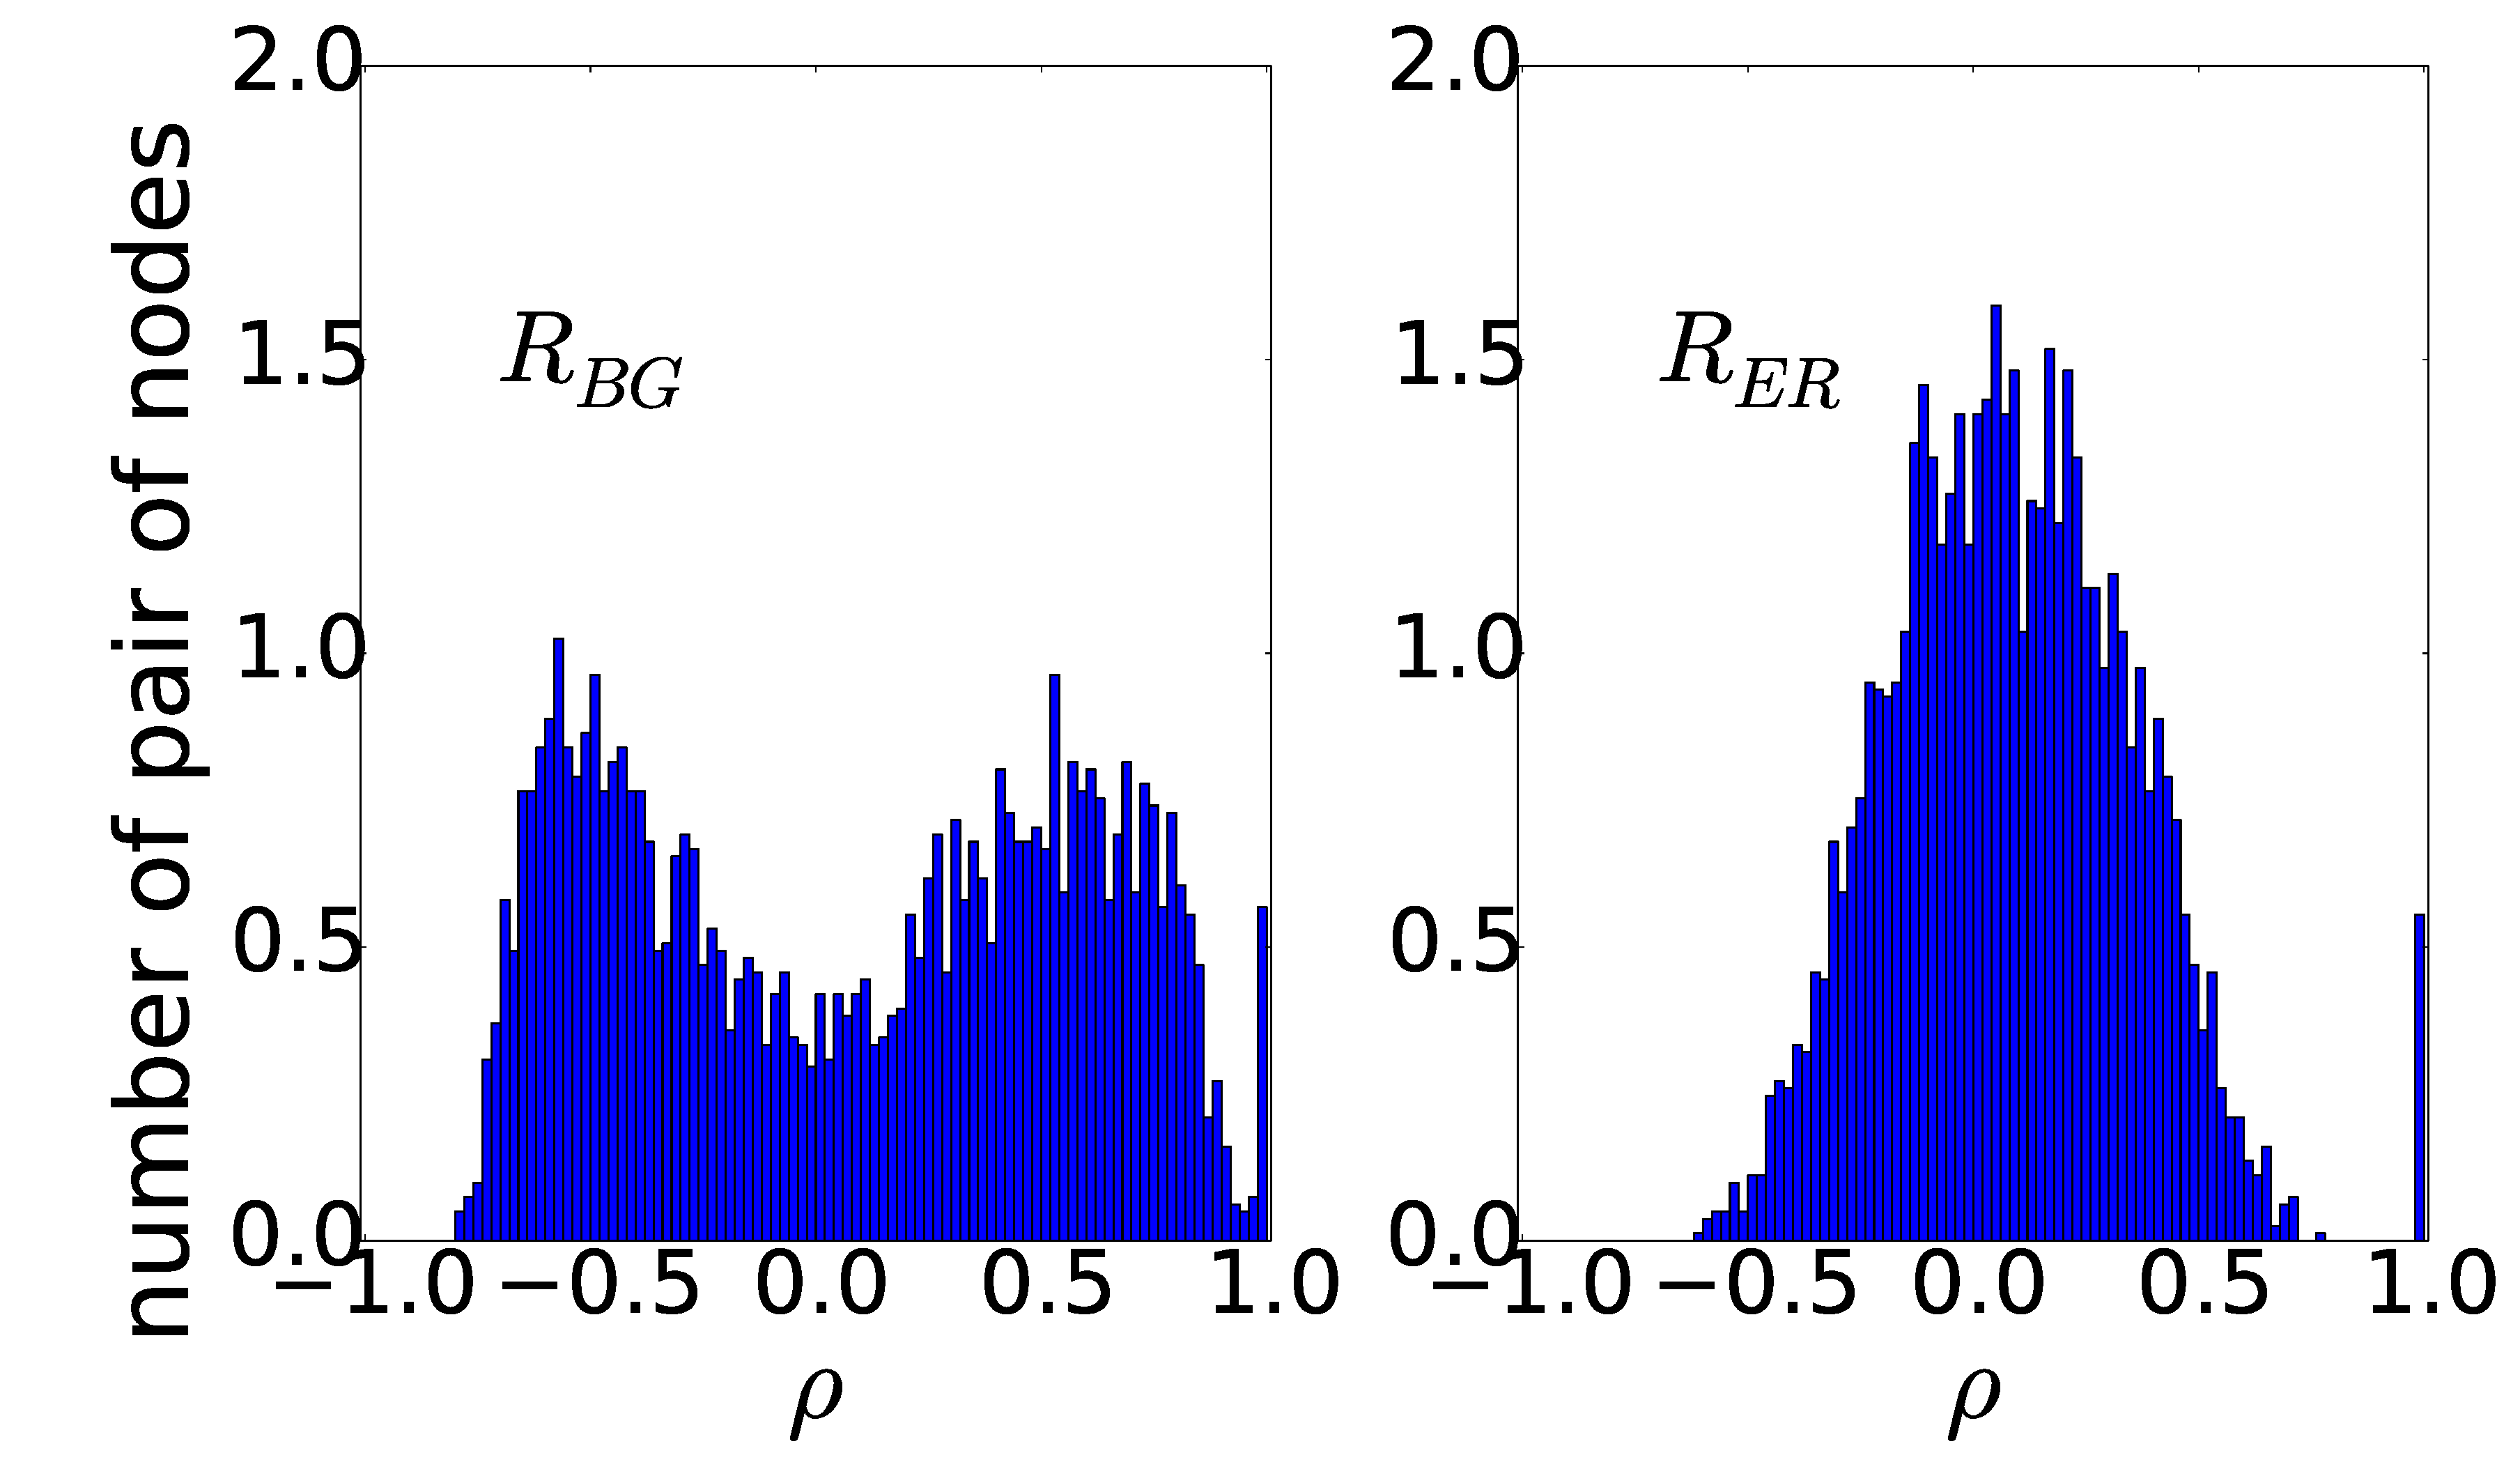
\includegraphics[width=0.48\textwidth]{Figures/histo_r_054_v_3_c_005_fhn} 
	 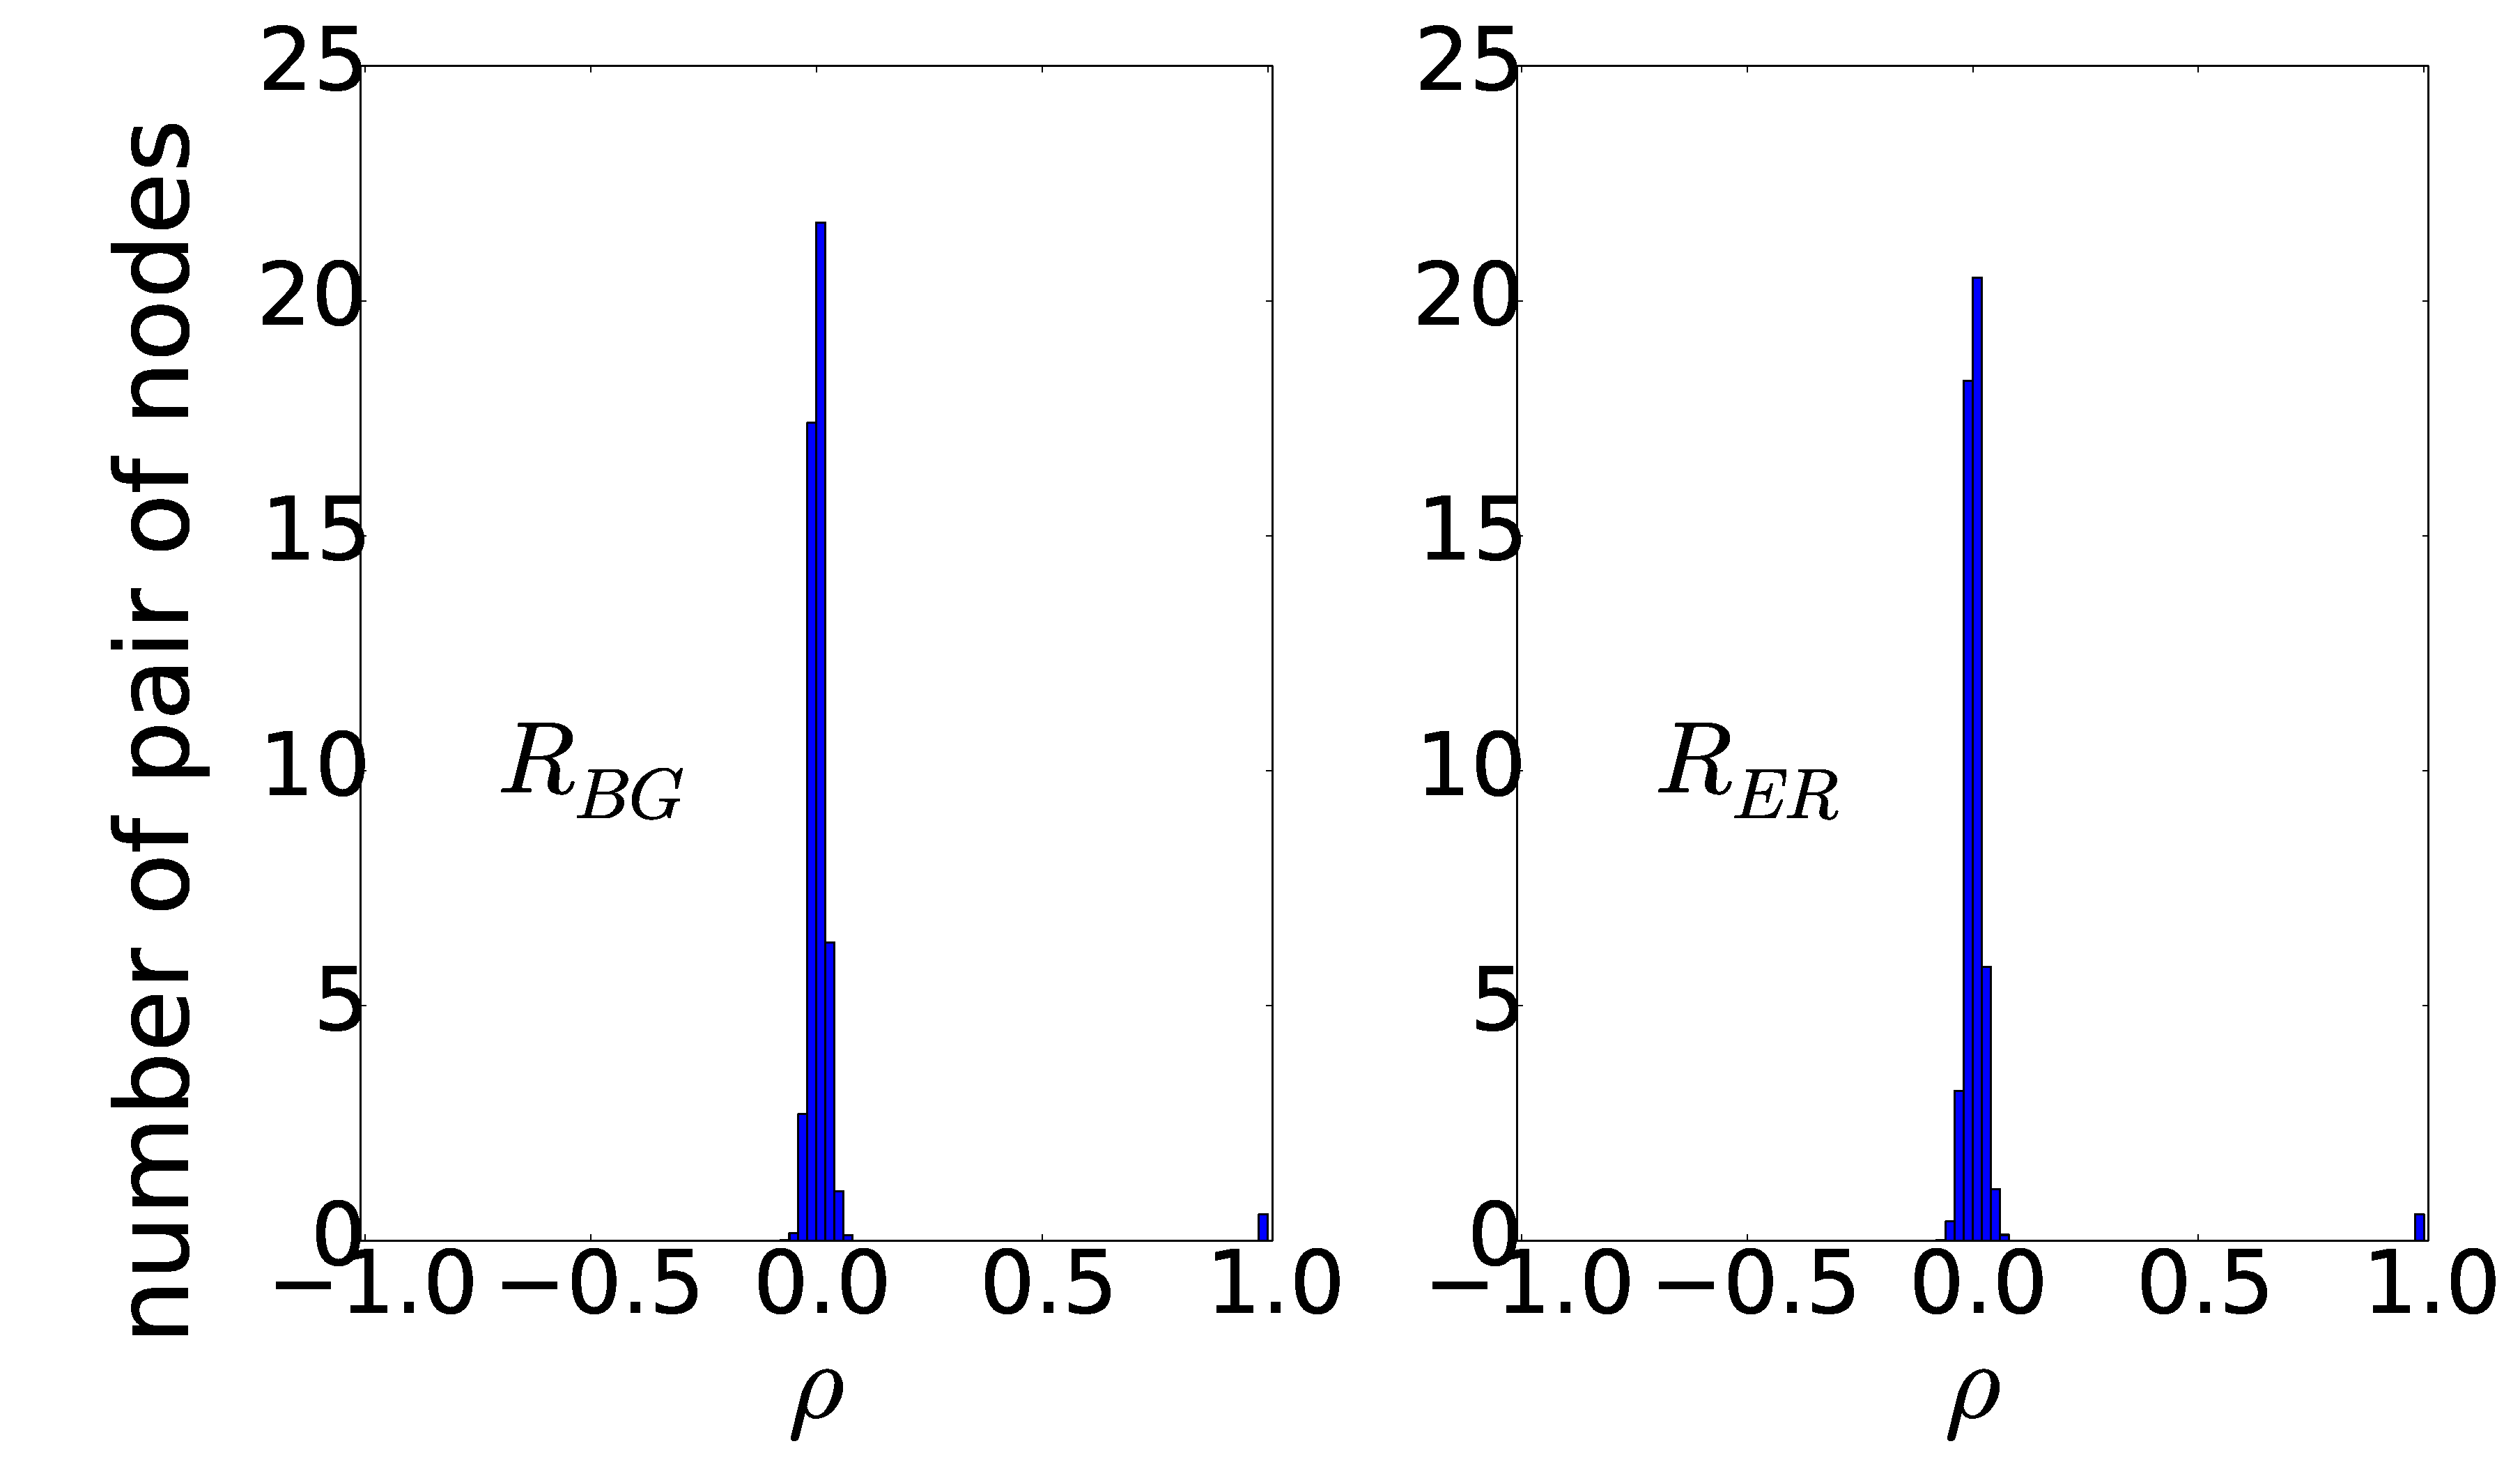
\includegraphics[width=0.48\textwidth]{Figures/histo_r_054_v_3_c_0005_fhn} 
   	 \caption{Two exemplary histograms chosen from red color from the cold color in Figure~\ref{fig:BG_vs_RG_v_3}
exhibiting strong differences ($c=0.05$, left) and strong similarity ($c=0.005$, right). Parameters as in
Fig~\ref{fig:BOLD_e_s}.} 
    \label{fig:histo_ex_v_3}
\end{figure} 

Figure~\ref{fig:histo_ex_v_3} illustrates exemplary histograms for $R_{BG}$, which is constructed on an
adjacency matrix obtained at $p=0.54$ given AC map, and for a corresponding random graph $R_{ER}$. The frequency of
the $\rho_{i,j}$ values in $R_{BG}$ resembles a bimodal distribution almost symmetric to zero for  $c=0.05$ (left),
indicating the presence of both correlated and anti-correlated node pairs in terms of their FHN modeled
time series. In contrast, $R_{ER}$ is centered around zero. The peaks at $\rho=1.0$ in each graph corresponds to
self-paired nodes, i.e. $\rho_{i,i}=1.0$.  For a small coupling strength ($c=0.005$, right), there are almost no
correlation visible.

\section*{Conclusion}
In this study, we have simulated resting-state functional connectivity in the human brain based on structural and
randomized networks. We have found an agreement between the numerical and empirical functional connectivity in
dependence on the network density and coupling strengths.
% We showed that it is possible to capture traces of measured BOLD fluctuations by modeling the anatomical connectivity
% map. The BOLD signals arising from changing neuronal activity are affected by the anatomical connectivity in the cortex.
We have also addressed the topological characteristics of brain graphs, which are built on structural connectivity data,
as well as random graphs of Erd\H{o}s-R\'{e}nyi type.
Moreover, the analogy between brain and random networks has been analyzed by comparing their modeled temporal
dynamics.  We have demonstrated that the simulated neuronal time series of brain graphs are clearly distinguishable
from that of random networks at relatively low coupling strengths $c$ and reasonable connection probability ranges $p$. 
 
% \reg{Concluding sentence still missing.}

\section*{Acknowledgments}
This study was assisted by BMBF (grant no. 01Q1001B) in the framework of BCCN Berlin (Project B7). We would like to
thank John-Dylan Haynes and his group for helpful discussions concerning the fMRI data analysis and Yasser
Iturria-Medina for sharing the DW-MRI data used in this work. \c{S}eyma Bayrak acknowledges additionally the support by
Jochen Braun.

\bibliography{sample}
% \newpage

\section*{Appendix}
\subsection*{Network Characterizations}
A network can be statistically described in terms of its topology, i.e. solely in terms of its connectivity and
independently of spatial positions of nodes and edges. In this work, it is aimed to characterize the topology of
$R_{BG}$ together with $R_{ER}$.   

\paragraph{Network Density}

The \textit{average degree} $\langle k \rangle$ of a network is proportional to the ratio of total number of edges $L$ to total number of nodes $N$ in a graph, 

\begin{equation}
\langle k \rangle = \frac{2L}{N}.
\end{equation}

The \textit{density} $\kappa$ of a network is formulated as the ratio between $L$ and maximum number of possible edges $\binom{N}{2}$,

\begin{equation}
\kappa = \frac{2L}{N(N-1)}.
\end{equation}	

The measure of network density can be referred to as the total \textit{wiring cost} of the network \citep{RUB10}. The \textit{degree} of an individual node $k_i$, average degree  $\langle k \rangle$ and network density $\kappa$ are key scalar measures to characterize the topology of a network. 

\paragraph{Average Clustering Coefficient}

The \textit{average clustering coefficient} $C$ of a network is calculated through individual clustering coefficients $C_i$ of single nodes,

\begin{equation}
C = \frac{1}{n} \sum\limits_{i\epsilon N}C_i = \frac{1}{n}\sum\limits_{i\epsilon N} \frac{2t_i}{k_i(k_i -1)} .
\end{equation} 

where $t_i$ is the number of triangles around node $i$ \citep{WAT98}. The clustering coefficient $C_i$ of a node $i$ is a measure of local connectivity and is highly correlated with the local efficiency of the information transfer \citep{LAT01}. The average clustering coefficient $C$ is a normalized version of $C_i$ for the whole network, yielding now a global property. $C$ is a measure of segregation, that is, the ability for specialized processing to occur within densely interconnected groups of brain regions \citep{RUB10}. It reveals how the individual nodes in a graph cluster together; how many neighbors of a node are neighbors of each other. 


\paragraph{Small-Worldness}

A small world network is both highly segregated and integrated, a measure of small worldness $S$ was proposed to capture this effect in a single statistic,

\begin{equation}
S = \frac{C/C_{rand}}{L/L_{rand}}, \,\,\,\,\,\,\,\,\,\,\,\,\,\,\,\,\,\,\,\,\,\,\,\,\,\,\,\,\,\,\,\,\,\,\,\,\,\,\,\, L = \frac{1}{n}\sum\limits_{i \epsilon N} L_i = \frac{1}{n}\sum\limits_{i \epsilon N} \frac{\sum\limits_{j \epsilon N, j \neq i }s_{ij}}{n-1 } \,\, .
\end{equation}
 
where $C$ and $C_{rand}$ are clustering coefficients, $L$ and $L_{rand}$ are characteristic path lengths of the original and random network respectively \citep{HUM08}. The random network here is constructed with \textit{Erd\H{o}s-R\'{e}nyi} method, which has the same number of nodes and links as the reference graph. $L$ is calculated through the shortest path length $s_{ij}$ between nodes $i$ and $j$, a basis for measuring integration \citep{RUB10}. 


\subsection*{Automated Anatomical Labeling}

Table \ref{tab:AAL} shows the Automated Anatomical Labeling (AAL) for the cortical and sub-cortical brain regions \citep{TZO02}. The brain is partitioned into $N=90$ regions symmetrically. AAL regions with index $n={1,2,...,45}$ lie on the right $R$ hemisphere, whereas $n={46,47,...,90}$ on the left $L$. The middle column of table describes the position of AAL regions anatomically in the cortex, and the last column corresponds to abbreviations.

\begin{table}[htbp] 
\centering
\caption[Automated Anatomical Labeling for the Brain Regions]{\label{tab:AAL}Anatomical Description of Brain Nodes }

\begin{tabular}{l | l | c}

Index R/L & Anatomical Description & Label \\ \hline  \hline 
  1/46 & Precentral & PRE   \\ 
  2/47 & Frontal Sup & F1 \\
3/48 & Frontal Sup Orb    &      F10 \\
4/49 & Frontal Mid        &       F2\\
5/50 & Frontal Mid Orb    &      F20\\
6/51 & Frontal Inf Oper   &    F30P\\
7/52 & Frontal Inf Tri    &     F3T\\
8/53 & Frontal Inf Orb    &      F30\\
9/54 & Rolandic Oper      &      RO\\
10/55 & Supp Motor Area  &      SMA\\
11/56 & Olfactory          &      OC\\
12/57 & Frontal Sup Medial  &   F1M\\
13/58 & Frontal Mid Orb     &   SMG\\
14/59 & Gyrus Rectus         &    GR\\
15/60 & Insula              &      IN\\
16/61 & Cingulum Ant       &   ACIN\\
17/62 & Cingulum Mid        &  MCIN\\
18/63 & Cingulum Post        & PCIN\\
19/64 & Hippocampus         &    HIP\\
20/65 & ParaHippocampal     &  PHIP\\
21/66 & Amygdala           &  AMYG\\
22/67 & Calcarine          &       V1\\
23/68 & Cuneus             &        Q\\
24/69 & Lingual            &   LING\\
25/70 & Occipital Sup      &       O1\\
26/71 & Occipital Mid      &       O2\\
27/72 & Occipital Inf      &       O3\\
28/73 & Fusiform           &    FUSI\\
29/74 & Postcentral        &   POST\\
30/75 & Parietal Sup       &       P1\\
31/76 & Parietal Inf       &       P2\\
32/77 & Supra Marginal Gyrus  &  SMG\\
33/78 & Angular               &   AG\\
34/79 & Precuneus             &   PQ\\
35/80 & Paracentral Lobule    & PCL\\
36/81 & Caudate               & CAM\\
37/82 & Putamen               & PUT\\
38/83 & Pallidum              &  PAL\\
39/84 & Thalamus              & THA\\
40/85 & Heschi                &  HES\\
41/86 & Temporal Sup          &    T1\\
42/87 & Temporal Pole sup     &  T1P\\
43/88 & Temporal Mid          &    T2\\
44/89 & Temporal Pole Mid     &  T2P\\
45/90 & Temporal Inf          &    T3\\
\hline  
  \hline 
\end{tabular}
\end{table}

\clearpage
%\reg{Still unclear, which and how the results for $v=3$m/s and $v=6$m/s can be explained and presented.}

\begin{figure}[htp] \centering
	 \includegraphics[width=0.49\textwidth]{Figures/Random_ACM_PA_task_v_6_FHN_01.eps} 
	 \includegraphics[width=0.49\textwidth]{Figures/Random_ACM_PA_task_v_6_BOLD_01.eps} 
   	 \caption{Statistical comparison of brain graphs $R_{BG}$ and random graphs $R_{ER}$ in terms of their
modeled temporal dynamics: FHN network model (left) and modeled BOLD activity (right). The heat map represents the
degree of similarity $d\left(H_{BG}, H_{ER}\right)$ between histogram distributions of simulated functional connectivity
of $R_{BG}$ and $R_{ER}$. Parameters as in Fig~\ref{fig:BOLD_e_s}, only with a different signal propagation velocity, here $v=6$ m/s.\\
%\red{What is the value of $v$ here?}
} 
    \label{fig:BG_vs_RG}
\end{figure} 

%\begin{figure}[htp] \centering
%	 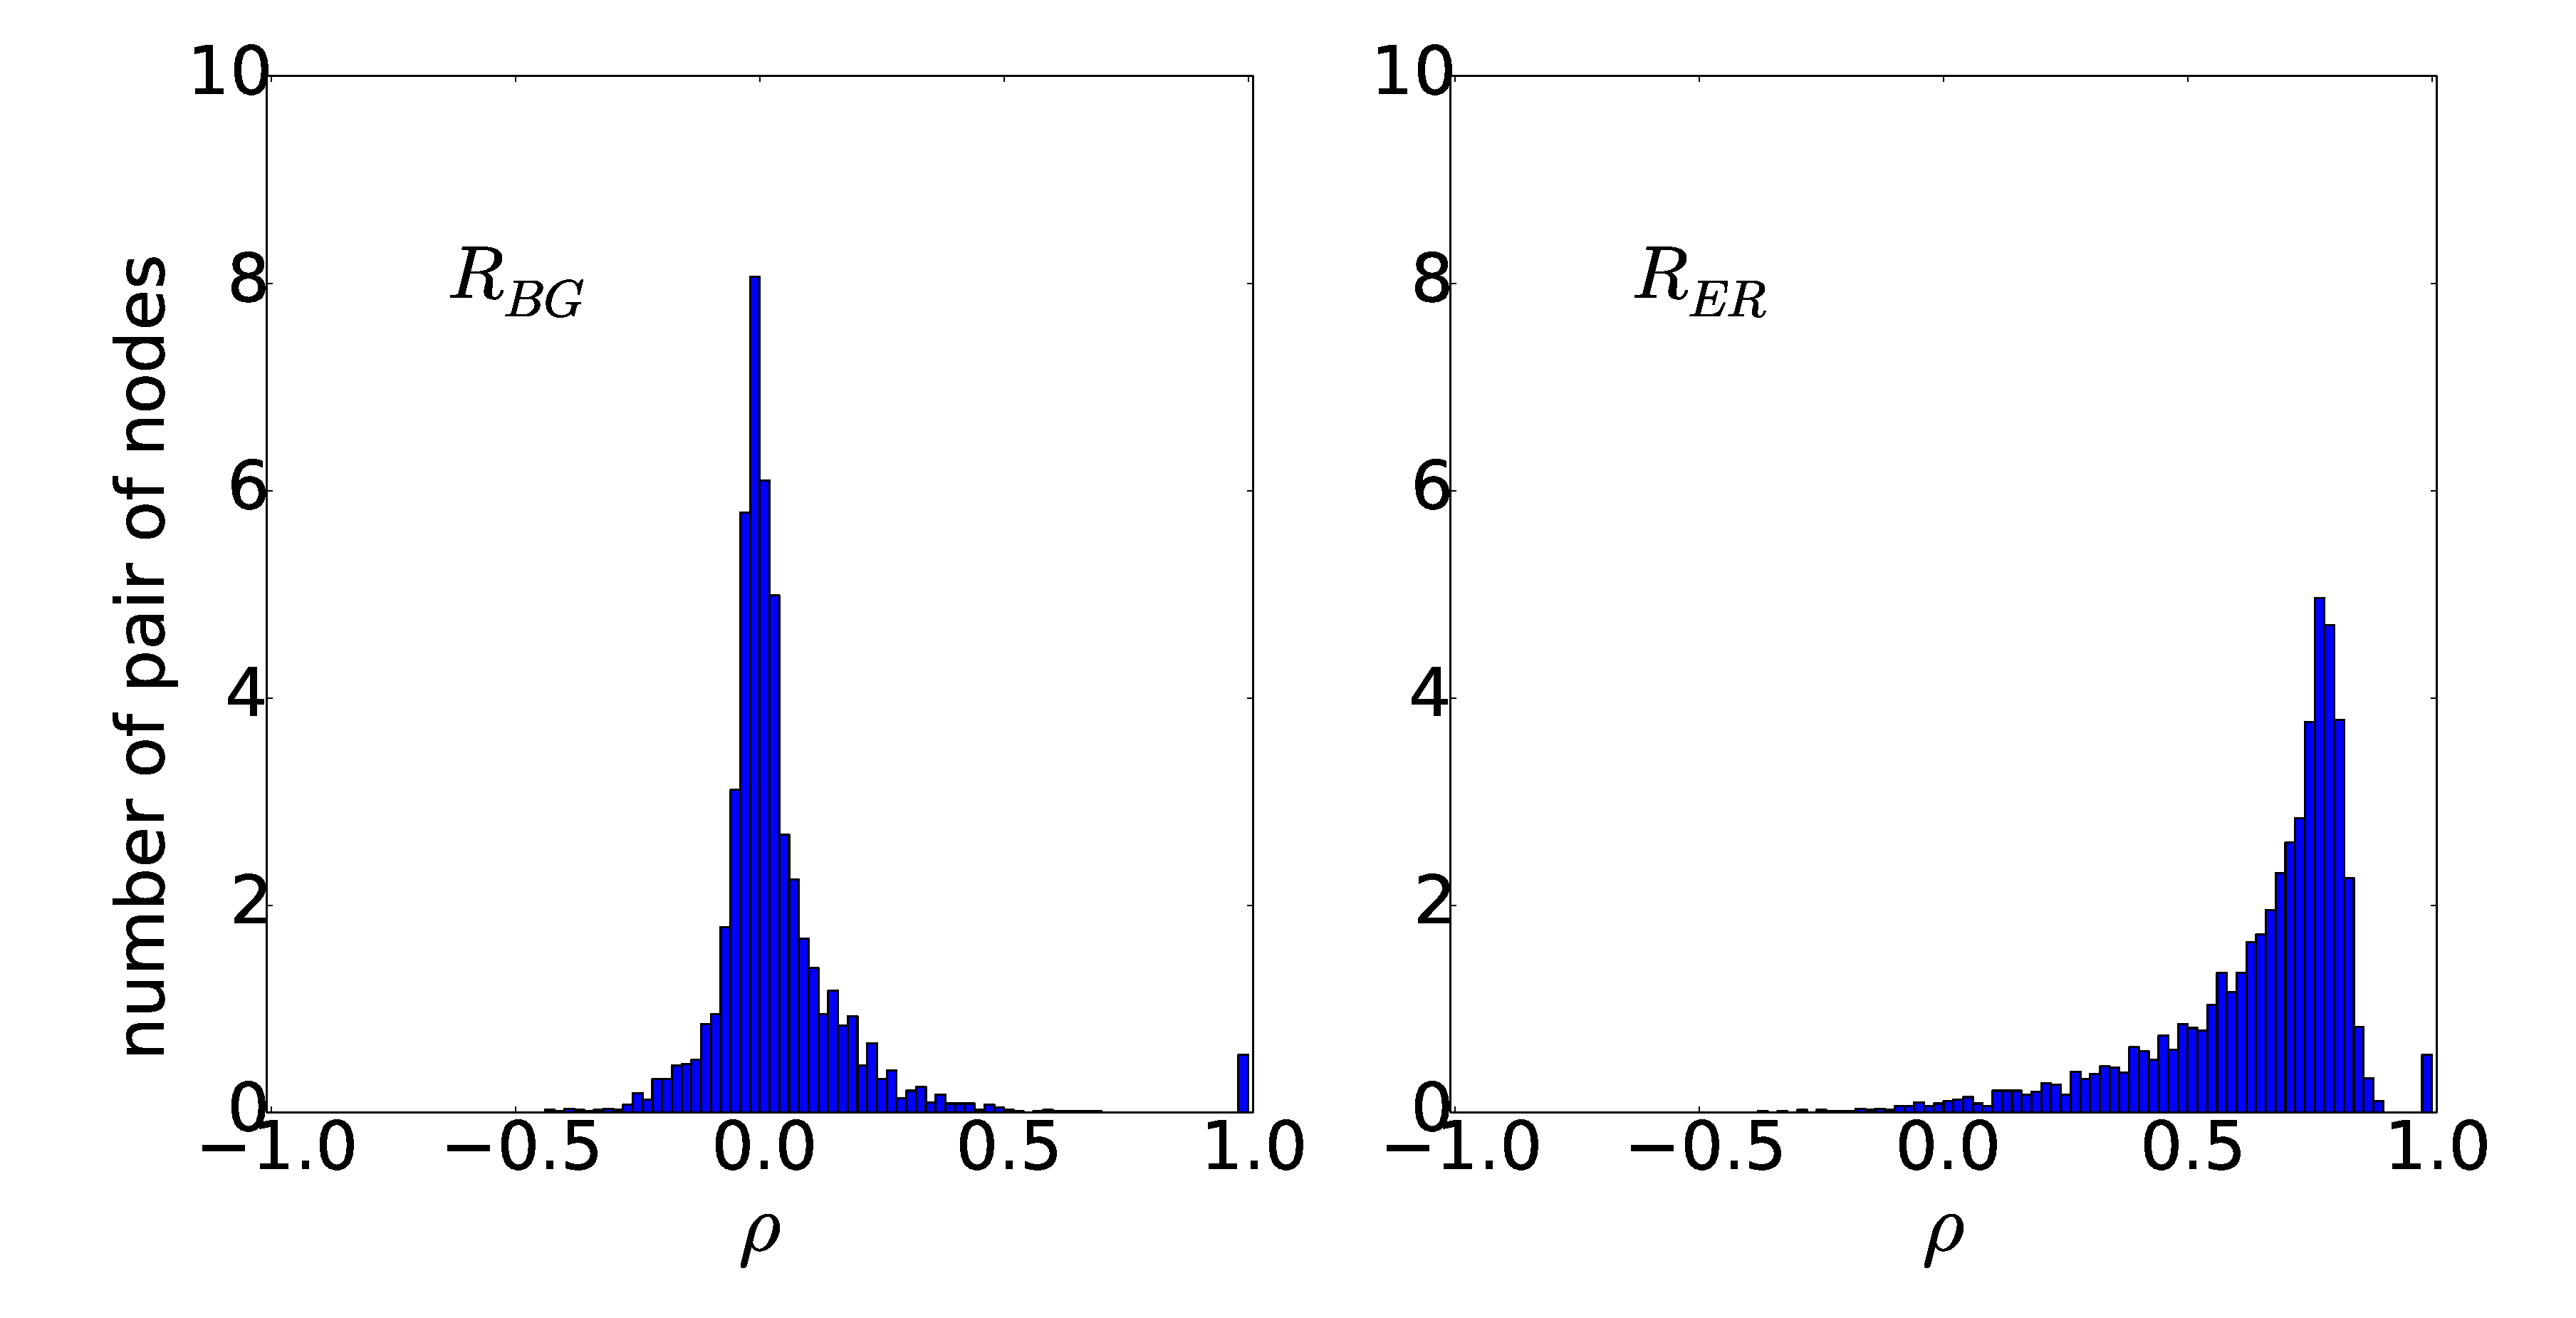
\includegraphics[width=0.85\textwidth]{Figures/Random_ACM_histo_taks} 
%   	 \caption{Histograms for the distribution of Pearson correlation coefficients $\rho$ among all possible pairwise
%combinations of nodal time series in $R_{BG}$ (left) and $R_{ER}$ (right). The FHN network parameters for the chosen
%distributions are $c=0.03$ and $v=6$ m/s, the network topology parameter is $p=0.54$.\\
%\red{Since this figure was obtained for $v=6$m/s, it should not be included.}} 
%    \label{fig:histo_ex}
%\end{figure} 

\end{document}